\documentclass[a4paper]{project}

\usepackage{graphicx}
\usepackage{float}
\usepackage{parskip}
\usepackage{geometry}
\usepackage[linesnumbered, ruled]{algorithm2e}
\usepackage{array}
\usepackage{listings}
\usepackage{xcolor}
\usepackage{amsmath}
\usepackage{multirow}
\usepackage{varioref}
\usepackage[pdfauthor={
	Natalia Spence (nas97),
	Niall Perry (nip33),
	Francesca Sasso (frs30),
	Reema Fraser (ref17),
	Abdullah Al-Samarrai (aba115),
	Joe Ball (job130),
	William Shipp (wis40),
	Prem Sharma (prs49)
}, pdftitle={Software Engineering Group Project}, pdftex, hidelinks]{hyperref}
\usepackage{cleveref}


% Preamble

% Numbering on subsubsections
\setcounter{secnumdepth}{3}

% Comments for pseudocode
\SetKwComment{tcp}{// }{}
\newcommand\commentfont[1]{\textcolor{blue}{#1}}
\SetCommentSty{commentfont}

% Extend footnote rule
% \renewcommand\footnoterule{%
	%  	\kern-3\p@
	% 	\hrule\@width \textwidth
	% 	\kern2.6\p@}
% \makeatother
% \makeatother

% Colour definitions
\definecolor{codegreen}{rgb}{0,0.6,0}
\definecolor{codegrey}{rgb}{0.5,0.5,0.5}
\definecolor{codepurple}{rgb}{0.58,0,0.82}
\definecolor{backcolour}{rgb}{0.95,0.95,0.92}

% Code style definition
\lstdefinestyle{code}{
	language=java,
	tabsize=4,
	commentstyle=\color{codegreen},
	backgroundcolor=\color{backcolour},
	keywordstyle=\color{magenta},
	numberstyle=\tiny\color{codegrey},
	stringstyle=\color{codepurple},
	basicstyle=\ttfamily, 
	breakatwhitespace=false,
	breaklines=true,
	numbers=left,
	numbersep=5pt,
	gobble=20,
	showstringspaces=false,
	captionpos=t
}
\lstset{style=code}

% Used by \maketitle on the title page	
\title{Software Engineering Group Project}
\subtitle{Design Document}
\shorttitle{Design}
\version{1.2}
\status{Release}
\date{26 March 2025}
\author{
	Natalia Spence (nas97),
	Niall Perry (nip33),
	Francesca Sasso (frs30),
	Reema Fraser (ref17),
	Abdullah Al-Samarrai (aba115),
	Joe Ball (job130),
	William Shipp (wis40),
	Prem Sharma (prs49)
}

\begin{document}
	\maketitle
	\tableofcontents
	
	\newpage
	
	\section{INTRODUCTION}\label{sec:introduction}
	
		\subsection{Purpose of this Document}\label{subsec:purpose}
		
			This document aims to provide a comprehensive overview of the design and architecture of Group 06's Deck of Cards project, developed for the Software Engineering module at Aberystwyth University in 2025.
		
		\subsection{Scope}\label{subsec:scope}
		
			The document details the system architecture, including package breakdowns, system interactions, and visual representations such as package, class, and sequence diagrams. Additionally, it contains drafts of pseudocode for complex functions, the majority of which can also be found in GitLab issue comments. While prior familiarity with the DS1 plan \cite{DS1} is not required, it is recommended for additional context. However, this document assumes that the reader is knowledgeable about the SE.QA.05 \cite{SE.QA.05} Design Standards and the Product Backlog \cite{Product Backlog}.
		
		\subsection{Objectives}\label{subsec:objectives}
		
			The primary objective of this document is to clearly present the system’s architecture, package structure, and key pseudocode components. It aims to illustrate how the various system components interact and justify the chosen package structure to enhance code readability and maintainability. This document serves as a foundation for developing a system that is both adaptable and well-structured.
		
		\clearpage
	
	\section{STATIC ARCHITECTURE DESCRIPTION}\label{sec:static-architecture-description}
	
		\subsection{Programs in the System and their Deployment}\label{subsec:programs-in-the-system-and-their-deployment}
		
			\subsubsection{Systems Diagram}\label{subsubsec:systems-diagram}
			
				\begin{figure}[ht]
					\centering
					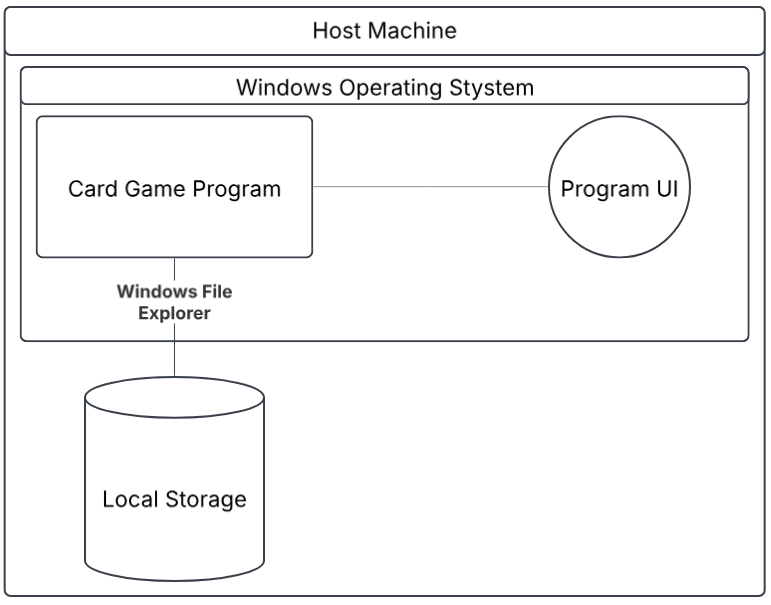
\includegraphics[width=\textwidth]{assets/systems-diagram.png}
					\caption{The Systems Diagram}
					\label{fig:system-diagram}	
				\end{figure}
			
			\subsubsection{Systems Architecture}\label{subsubsec:systems-architecture}
			
				The system architecture comprises three primary components that interact on the host machine to execute the program: the program engine, the user interface (UI), and local storage.
				
				The program engine is responsible for executing the card game’s core logic. It manages game mechanics, processes user inputs, and controls the overall flow of the application. The engine also integrates with JavaFX, which facilitates the user interface UI — the second key component. The UI provides a graphical representation through which users can interact with the program, enabling input and engagement with the game.
				
				The third component is the local storage of the host machine, which is used to store essential assets such as card and table images, as well as game and dealing layout recordings. The program engine accesses this storage through the host operating system’s built-in file management capabilities, such as Windows File Explorer for Windows.
				
				All three components operate locally on a single host machine, with no requirement for external network access to ensure full program functionality.
		
		\subsection{Package Diagram}\label{subsec:package-diagram}
		
			\begin{figure}[ht]
				\centering
				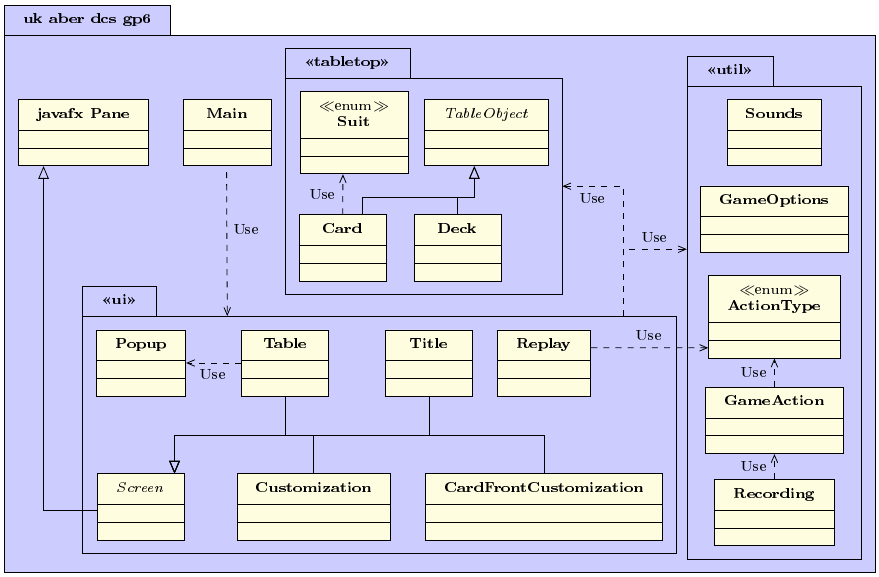
\includegraphics[width=0.8\linewidth]{assets/Package_diagram.png}
				\caption{The Package Diagram}
				\label{fig:package-diagram}
			\end{figure}
		
			\subsubsection{Package Architecture}\label{subsubsec:package-architecture}
			
				The packages in the design of the program are split into three groups:
				
				1) \textit{ui} - Manages the user interface, including displaying contents on the window and receiving user input.
				
				2) \textit{tabletop} - The data structures that ensure the program can actually function, including the cards and decks.
				
				3) \textit{util} - Various other utility classes used for other purposes, such as recording games, playing sound effects or saving files for custom images. These essentially act as controllers for everything that isn't ui or data structure related.
				
				\textbf{Package Interactions}
				
				The \textit{ui} package is the most prominent aspect of the application, with every screen involved in the program being contained within. All display and user interaction occurs within the \textit{ui} package, which in turn communicates with both other packages to cause changes in the system, and the content displayed by the \textit{ui} package.
				
				The tabletop package is the core of the system, where the actual data structures are located, and is often used by the ui package to allow the program to function. Without it, you would have a window but the core program itself would not exist. Any direct manipulation of these data structures (aside from their positions on the UI) is located here.
				
				Finally, the \textit{util} package contains the other useful classes required for the program to operate. The \textit{ui} package will regularly interact with the \textit{util} package for important functionality that's not directly occurring on the UI, such as recording games, playing sound effects, saving user settings and loading user images.
			
			\clearpage
		
	\section{STATIC DESCRIPTION}\label{sec:static-description}
		
		\subsection{Class Diagrams}\label{subsec:class-diagrams}
		
			\begin{figure}[H]
				\centering
				
\includegraphics[width=\linewidth]{"assets/class-diagram-ui.png"}
				\caption{The Class Diagram for the ui Package}
				\label{fig:class-diagram-ui}
			\end{figure}
			
			\pagebreak
			
			\subsubsection{Screen}\label{subsubsec:screen}
			
				$Screen$ is an abstract base class for all UI screens in the game. It defines the essential methods each screen must implement, such as initializing UI elements, displaying the screen, handling events, and reacting to key inputs. It also includes a helper method to switch between screens. Here are some of its functions:
			
				\begin{itemize}
					\item Screen(): Constructor that initializes a screen by calling abstract methods initializeScreen() and initializeEvents() to set up UI elements and event handlers.
					\item changeScreen(Screen current, Screen next): Switches the current screen to a different one. If moving from CardFrontCustomization to Table, it also sets the number of decks before displaying the new screen.
					\item initializeScreen() (abstract): Must be implemented by subclasses to add and configure UI components for the screen.
					\item displayScreen() (abstract): Called every time the screen is shown. Subclasses use this to layout and update UI components based on window size.
					\item initializeEvents() (abstract): Subclasses implement this method to register event listeners and filters, such as mouse or button actions.
					\item keyPressed(KeyEvent keyEvent) (abstract): Handles keyboard input specific to the screen (e.g., tab navigation, confirmation via Enter).
				\end{itemize}
				
			\subsubsection{Title}\label{subsubsec:title}
				
				The $Title$ class is rather small and simply handles the title screen. \\
				It has a small number of attributes and methods, the former are listed below:
				
				\begin{itemize}
					\item Instance: the instance of the Title screen
					\item titleText: the program name text displayed at the top of the screen
					\item startButton: the button to go into the Customization screen to start the game
					\item replayButton: the button to open a file chooser to play a replay file
					\item quitButton: the button to quit the program
					\item stage: the JavaFX stage, used for the replay file chooser
				\end{itemize}
				
				The methods involved are consistent with the rest of the screens:
				
				\begin{itemize}
					\item Title: the constructor, creates the title screen
					\item setStage: sets the JavaFX stage, used for the file chooser for replays
					\item initializeScreen: creates all components to be displayed on the screen
					\item displayScreen: actually displays the screen, setting the size and position of components
					\item initializeEvents: sets up all the event handlers required to interact with the screen
					\item showInvalidFilePrompt: shows a prompt with an error when an invalid replay file is selected
					\item keyPressed: handles keyboard input
					\item getInstance: gets the Title instance
				\end{itemize}
			
			\subsubsection{Customization}\label{subsubsec:customization}
			
				The $Customization$ class handles the user interface for setting up visual preferences.
				
				\begin{itemize}
					\item Allows users to select custom card and table images
					\item Lets users choose the number of decks and jokers
					\item Uses JavaFX UI elements for interactive customization
					\item Called before starting or replaying a game
				\end{itemize}
			
			\subsubsection{CardFrontCustomization}\label{subsubsec:cardfrontcustomization}
			
				The CardFrontCustomization class represents a user interface screen that allows players to customize the front face of their playing cards by selecting a card number, suit, and uploading custom images. It follows the singleton pattern to ensure only one instance exists, and it integrates mouse and keyboard interaction to facilitate navigation and customization. \\
				The attributes of this class are:
			
				\begin{itemize}
					\item CardFrontCustomization(): Private constructor to enforce the singleton pattern. Ensures only one instance of this screen exists.
					\item initializeScreen(): Sets up all UI elements including card preview, suit icons, navigation buttons, and layout groups on the screen.
					\item displayScreen(): Configures the layout and appearance of the screen, initializes the card preview with default settings, and loads images for suits and the card front.
					\item loadImage(String path): Loads an image from a given resource path and returns it, or logs a warning and returns null if not found.
					\item loadImage(String primaryPath, String fallbackPath): Attempts to load an image from the primary path, falls back to a secondary path if the first fails.
					\item setUpSuitImage(Image suitImage, Rectangle suitShape, double xPos): Sets image and position for a suit rectangle (clubs, hearts, etc.) used in the UI.
					\item setUpLayoutClusters(): Binds UI element positions to the screen’s size for responsive layout design.
					\item updateCardNumberPosition(): Re-centers the card number text between the navigation arrows based on current layout bounds.
					\item initializeEvents():Attaches mouse click event handlers for suit selection, card image updates, navigation arrows, and screen navigation buttons.
					\item updateCurrentFront(GameOptions options): Updates the card front preview with the selected suit and number image, falling back to default if user-customized image isn't found.
					\item updateCardNumberDisplay(int difference, GameOptions options): Changes the current card number and updates its corresponding label (e.g., "Ace", "Jack", "10").
					\item allowCurrentBorderOnly(Rectangle obj): Highlights the selected suit by giving it a colored border and removes it from others.
					\item keyPressed(KeyEvent keyEvent): Handles keyboard navigation (Tab, Shift+Tab, Escape, and Enter) between UI elements on the screen.
					\item setCardNumber(Text text): Sets the internal cardNumber Text object.
					\item setSuit(Text text): Sets the internal suit Text object.
					\item getCardNumber(): Returns the current card number Text object.
					\item getSuit(): Returns the current suit Text object.
					\item getCardNumberDisplayed(): Returns the Text object displaying the card number label (e.g., "King").
					\item getInstance(): Provides access to the singleton instance of this class.
				\end{itemize}
				
			\subsubsection{Table}\label{subsubsec:table}
				
				$Table$ is the core interactive UI screen in the card game that allows users to interact with cards and decks. It handles rendering, mouse/keyboard events, replay controls, pop-ups, layout management, and deck/card manipulation. It's implemented as a singleton and extends the abstract $Screen$ class.
			
				\begin{itemize}
					\item Table(): Private constructor to enforce singleton pattern.
					\item getInstance(): Returns the single instance of the Table.
					\item initializeScreen(): Creates and adds all UI components including menu, action bar, and selection rectangle.
					\item displayScreen(): Renders all visual components, background image, menu options, dialog boxes, and handles replay UI states.
					\item initializeEvents(): Attaches all necessary mouse event handlers for object interaction and menu toggling.
					\item keyPressed(KeyEvent): Handles keyboard shortcuts for moving, rotating, flipping, and manipulating selected objects or UI navigation.
					\item setStartDecks(int deckCount): Adds and positions the specified number of decks to the table.
					\item displayTableObject(TableObject): Adjusts the size, image, and layout of a Card or Deck on the table.
					\item loadCardImages(Card): Loads customized or default front/back images for a given card.
					\item addEventHandlersForTableObject(TableObject): Adds full interactivity (click, drag, rotate, hover) to a card or deck.
					\item addEventHandlersForSpecificTableObject(TableObject): Adds specific handlers, e.g., right-drag to draw cards from decks.
					\item moveTableObject(MouseEvent, TableObject): Handles dragging logic for TableObjects and overlap checks.
					\item closePopups(): Closes all open right-click popups on the table.
					\item showSaveDialogBox(String): Displays a prompt for saving recordings or loading layouts.
					\item displaySaveDialogBox(String): Constructs and renders a save/load dialog box.
					\item getSaveDialogText(): Returns the prompt text from the currently visible dialog.
					\item addSaveDialogEventHandlers(ArrayList<Node>): Attaches logic to dialog box buttons.
					\item closeSaveRecordingDialogBox(ActionType): Closes the dialog and resets state based on the recording type.
					\item showMenuButton(): Displays the hamburger-style menu button in the UI.
					\item createTableMenuOptions(): Creates menu options like recording toggle, grid, and exit.
					\item getMenuButtonImage(int): Returns the image corresponding to a menu button number.
					\item setupMenuButton(Rectangle, ImageView, int): Adds functionality to each menu button (e.g., exit app or toggle layout recording).
					\item showTableMenu(): Displays or hides the table's dropdown menu.
					\item createActionBar(): Builds the UI components (buttons and text) for the replay control bar.
					\item getActionBar(): Returns the action bar group.
					\item displayReplayActionBar(boolean): Renders the replay controls (or prompts) based on the state.
					\item getActionBarButtonImage(int): Provides images for replay buttons (e.g., play, pause, skip).
					\item setupActionBarButton(Rectangle, ImageView, int): Assigns replay functions to buttons (play, pause, etc.).
					\item removeActionBar(): Removes the replay action bar from the screen.
					\item updateActionBarSpeedText(int): Updates the replay speed display text.
					\item resetTable(): Resets and reinitializes the table (used after replay ends).
					\item endDealingReplay() / isDealing(): Ends or checks whether dealing layout replay is active.
					\item setLongLayout(boolean) / isLongLayout(): Flags if a dealing layout exceeds deck capacity.
					\item setReplayMode(boolean): Sets replay mode state.
				\end{itemize}
			
			\subsubsection{Popup}\label{subsubsec:popup}
			
				The $Popup$ class generates menus for table objects when the user right-clicks a card or group.
				
				\begin{itemize}
					\item Displays options based on selected object(s) (e.g., flip, reveal, rotate)
					\item Built using JavaFX Group and Rectangle components for visual structure
					\item Enables actions to be applied to several selected cards or decks simultaneously
					\item Auto-closes when the user clicks elsewhere or selects an action
				\end{itemize}
				
			\subsubsection{Replay}\label{subsubsec:replay}
				
				The $Replay$ class manages the playback of previously recorded game sessions.
				
				\begin{itemize}
					\item Loads .csgr recording files and reads stored game actions
					\item Allows user to step forward or backward through actions
					\item Supports autoplay with adjustable speed
					\item Displays visual indicator when playback is complete
					\item Integrates with $Recording$ to interpret saved actions
				\end{itemize}
			
			\begin{figure}[H]
				\centering
				
\includegraphics[width=\linewidth]{"assets/class-diagram-tabletop.png"}
				\caption{The Class Diagram for the tabletop Package}
				\label{fig:class-diagram-tabletop}
			\end{figure}
			
			\subsubsection{TableObject}\label{subsubsec:tableobject}
			
				The $TableObject$ class acts as a base class for other objects on the game table. Its attributes are as follows:
				
				\begin{itemize}
					\item anchorX and anchorY: Table location reference for mouse movement
					\item prevX and prevY: Double that temporarily stores the previous X and Y locations respectively on the table of an object 
					\item Dragging: boolean that records whether an object is currently being moved by the mouse
					\item selectedObjects: a list of table objects that are currently selected by control-clicking
					\item hoveredTableObject: a tableObject that the mouse is currently hovering over
					\item draggedCard a tableObject that is currently being dragged by the mouse
					\item customID: a protected integer
					\item prevRotation: a double for storing the previous assigned rotation of a card before manipulation
				\end{itemize}
				
				The $TableObject$ Class has several methods to add functionality:
				
				\begin{itemize}
					\item A constructor to create a tableObject
					\item getSelectedObjects: returns the selectedObjects list of tableObjects
					\item toTableObject: creates a table object from a string of specific format
					\item objectsIsBeingDragged: returns the value of the variable dragging
					\item setDragging: setter for the variable dragging
					\item getHoveredTableObject: returns the table object stored in the variable hoveredTableObject
					\item setHoveredTableObject: sets the variable hoveredTableObject to the table object passed to this method
					\item Getter and Setters for the anchorX and anchorY variables
					\item Getter and setter for the draggedCard variable
					\item getCustomID: returns the integer value of the customID variable
					\item tableObjectsAreEqual: checks if two given tableObjects are equal returning a boolean based on the result
					\item Getter and setter for the prevRotation variable
					\item Getter and setter for the prevX and prevY variables
				\end{itemize}
				
			\subsubsection{Suit}\label{subsubsec:suit}
				
				The enumeration of $Suit$ provides the suits for the card class and some simple method for their use. \\
				These values include: HEART (H), DIAMOND (D), SPADE (S), CLUB ( C) and JOKER (J) with their corresponding shortHand representation. \\
				The methods provided in the $Suit$ Enum are:
				
				\begin{itemize}
					\item The constructor
					\item toString: returns the string representation of shortHand
					\item convertToSuit: Takes a ShortHand representation of a suit and returns the corresponding Enum value
				\end{itemize}
				
			\subsubsection{Card}\label{subsubsec:card}
				
				The $Card$ Class consists of several attributes:
				
				\begin{itemize}
					\item Suit: enum type that represents the card's suit (heart, diamonds, spades, clubs and joker)
					\item Index: integer value that represents the numerical value of the card as well as if it is a king, queen or ace
					\item isFaceUp: a boolean type that records if the card is face up (true) or face down (false)
					\item frontImage : the image to be displayed on the front of the card
					\item backImage  the image to be displayed on the back of the card
					\item createdCards: hash map
				\end{itemize}
				
				The $Card$ Class consists of several attributes:
				
				\begin{itemize}
					\item Two $Card$ constructor methods used throughout the program
					\item createCardID: creates a unique ID for every card
					\item getSuit: returns the suit of the card
					\item toString: creates a string representation of a unique card
					\item toCardString: creates a two letter string representation of a unique card
					\item toCard: converts a string in specific format to a card object
					\item flip: flips the card over to reveal hidden face
					\item isFaceUp: returns the isFaceUp boolean value
					\item flipStateOnly: flips the card without affecting the UI
					\item setBackImage: sets the image on the back of the card to the one provided to the function
					\item setFrontImage: sets the image on the Front of the card to the one provided to the function
					\item changeImage: used when flipping the card to help the appearance of a smooth transition to the other face
					\item rotateCard: Creates a rotation animation to spin the card around the Y-axis for the flipping animation
					\item revealCard: flips the card for 5 seconds to reveal the hidden face
					\item tableObjectsAreEqual: checks if two given cards have the same index, suit and face up
				\end{itemize}
				
			\subsubsection{Deck}\label{subsubsec:deck}
				
				This class represents a collection of $Card$s, offering methods for shuffling drawing and managing cards, its attributes are:
				
				\begin{itemize}
					\item drawnCard: a card type that stores the last card being drawn from the deck
					\item Cards: a list of card objects that are assigned to the deck
					\item cardCountText: text count of cards assigned to the deck
					\item deckCount: integer count of the decks currently created
					\item shuffleAnimation: a sequentialTransition used as an animation played during various operations on decks
				\end{itemize}
				
				The methods included in the $Deck$ class are:
				
				\begin{itemize}
					\item Three constructors for creating decks at various points in the program
					\item createDeckID: returns the next integer ID for a newly created deck based on the deckCount variable
					\item initializeDeck: sequentially adds all required cards to a newly created deck
					\item initializeCardCount: initializes a card count to be displayed in the corner of the deck on the UI
					\item unpackTableObject: forms a deck of cards from a list of tableObjects
					\item shuffleDeck: shuffles the cards within a selected deck, returns a boolean true when completed
					\item getAnimation: creates an animation to be used when shuffling and moving cards within a deck, the number of times the animation loops is set by the integer passed to the method, the final animation is assigned to the shuffleAnimation variable
					\item Getter for the Cards list
					\item setCardCountLocation: positions the card count UI element on the deck 
					\item Getter for the cardCountText
					\item toString: creates a string representation of a deck the deck and its unique ID and all the cards contained inside the deck in order
					\item loadRecordedDeckData: takes a string of specific format and creates a deck with accompanying cards, used for loading of recorded gameplay
					\item getTopCard: returns the card object at the top of the deck
					\item getDrawCard: returns the card object drawn from the deck
					\item setDrawnCard: sets the drawnCard variable to the given card object
					\item drawCard: moves the drawn card from the top of the deck to the table, if the deck has only one card once the top card is drawn the deck is replaced with the remaining card
					\item tableObjectsAreEqual: checks if two decks are equal, ignoring object identity and UI properties
					\item cloneDeckForReverse: creates a copy of the deck and removes the first card for use in replays
				\end{itemize}
				
				\clearpage
			
			\begin{figure}[H]
				\centering
				
\includegraphics[width=\linewidth]{"assets/class-diagram-util.png"}
				\caption{The Class Diagram for the util Package}
				\label{fig:class-diagram-util}
			\end{figure}
			
			\subsubsection{GameOptions}\label{subsubsec:gameoptions}
			
				The $GameOptions$ class stores the user’s game setup preferences and configuration settings.
				
				\begin{itemize}
					\item Stores configuration data such as number of decks, jokers, and custom image selections
					\item Provides getter and setter methods for values like deck count, joker count, and selected image paths
					\item Ensures customization settings stay within allowed limits, such as the maximum number of decks or jokers
					\item Includes toggle methods for features such as grid snapping and sound effects
				\end{itemize}
				
			\subsubsection{ActionType}\label{subsubsec:actiontype}
			
				ActionType is an enumeration that defines all the possible types of actions that can occur during gameplay or UI interaction. These actions are used by the game engine to record, replay, and interpret player behavior and system events such as card movements, layout changes, or recording control signals.
				
				\begin{itemize}
					\item shouldMerge: determines whether multiple of an action type in a row should be merged into one action during recording
				\end{itemize}
				
			\subsubsection{GameAction}\label{subsubsec:gameaction}
				
				The GameAction class models a single action taken during the game. It stores information about the type of action, the object involved (like a card or pile), and any relevant arguments (like coordinates). It's primarily used for saving, loading, and replaying game interactions. \\
				It’s functions are as follows:
				
				\begin{itemize}
					\item GameAction(ActionType actionType, TableObject actionObject, Map<String, Double> actionArgs): Protected constructor that initializes a new GameAction with its type, associated game object, and relevant action arguments.
					\item toString(): Returns a custom string representation of the action, combining its type, object data, and arguments—mainly used for saving or debugging.
					\item getActionObject(): Returns the TableObject (e.g., a card, pile, etc.) associated with this action.
					\item getActionArguments(): Returns a map of argument keys and their numeric values that define the specifics of the action (e.g., positions or sizes).
					\item toAction(String actionData): Static method that converts a string (typically from a saved file) back into a GameAction object, parsing the type, object, and arguments.
					\item getActionType(): Returns the ActionType enum value representing what kind of action this is (e.g., draw, move, place).
				\end{itemize}
			
			\subsubsection{Recording}\label{subsubsec:recording}
				
				The $Recording$ Class handles recording and loading replays and dealing layouts. \\
				Its attributes include:
				
				\begin{itemize}
					\item recordingLayout: a boolean, true if a game recording is currently in progress and false if not
					\item recordingGame: a boolean, true if a layout recording is currently in progress and false if not
					\item actionQueue: a queue of gameActions to be recorded
					\item recordedLayoutActions: a list of recorded layout actions
					\item recordedGameActions: a list of recorded game actions
					\item loadedGameActions: a list of gameActions loaded from a previous recording file
				\end{itemize}
				
				The methods provided with the class are as follows:
				
				\begin{itemize}
					\item Recording: the Constructor for the class
					\item clearRecordedActions: clears the recordedLayoutActions and recordedGameActions lists at the end of a recording ready for a new recording to start
					\item Getter for the loadedGameActions list
					\item Run: controls the recording process and contains the main recording thread, the method continues running as long as any recording is in progress
					\item recordAction: records a single GameAction to the appropriate list
					\item mergeActions: combines two GameActions into one to simplify the recording process
					\item createGameAction: creates a gameAction from an ActionType and a Tableobject, multiple game actions can be created if an action requires
					\item startRecordingGame: starts the recording of a game
					\item startRecordingLayout: starts the recording of a dealing layout
					\item startRecordingThread: creates the thread for the recording process to run on 
					\item toggleRecordingGame: toggles the game recording process on or off appropriately
					\item toggleRecordingLayout: toggles the layout recording process on or off appropriately
					\item saveInitialState: saves the initial state of all tableObjects and their locations
					\item saveRecordingFile: saves the recording file once a recording has been completed
					\item loadRecording: loads a previous recording from a specified file
					\item endAllRecordings: utilises the toggleRecordingLayout and toggleRecordingGame methods to end all running recordings
				\end{itemize}
				
			\subsubsection{SoundManager}\label{subsubsec:soundManager}
				
				SoundManager is a utility class for handling sound effects in the game. Currently, it manages and plays a sound effect when a card is selected, using JavaFX's AudioClip. cardSelectSound is a private static AudioClip object that loads the audio file ClickSoundTest.mp3 from the resources directory when the class is initialized. It is used to provide auditory feedback (e.g., when selecting a card). It’s playCardSelect() plays a short audio clip (ClickSoundTest.mp3) to give audio feedback when a card is selected or interacted with. Useful for enhancing user experience with sound cues.
		
		\subsection{Discussion of Key Data Structures}\label{subsec:discussion-of-key-data-structures}
		
			This section is incorrect (as of 26th March, 2025) and will be updated soon. The content below is a mix of out of date and just incorrect.
			
			The program uses a few key data structures to manage and organise data efficiently.
			
			These structures have different functionalities within the system, such as player customization and Game recording data.
			Listed below are the key data structures used throughout the program:
		
		\subsubsection{Player Customization}\label{subsubsec:player-customization}
		
			\begin{itemize}
				\item Attributes: This structure includes the decided card types and background the player(s) would like to use while playing the game.
				\item Functionality: This structure is important for the setup of game as it stays throughout and cannot be changed once decided.
				\item Implementation: This Structure is implemented as class and derived from the screen parent class where the setup is stored. 
			\end{itemize}
		
		\subsubsection{Game Recording Data}\label{subsubsec:game-recording-data}
		
			\begin{itemize}
				\item Attributes: This structure included being able to record and replay previous games that have been played in the past.
				\item Functionality: This Structure is important for making the game repeatable and re playable as the User is able to watch previous setups and rules to follow along to.
				\item Implementation: This Structure is implemented as a class and derived from the Table parent class where a loading file is created, stored and ran upon request
			\end{itemize}
		
		\subsection{Mapping from User Stories to Classes}\label{subsec:mapping-from-user-stories-to-classes}
		
			{
				\centering
				\begin{tabular}{|l|l|}
					\hline
					\textbf{Requirement}             & \textbf{Classes Providing Requirement}             \\ \hline
					US1 Number of Decks              & Customization, GameOptions                         \\ \hline
					US2 Number of Jokers per Deck    & Customization, GameOptions                         \\ \hline
					US3 Card Images                  & Customization, CardFrontCustomization, GameOptions \\ \hline
					US4 Table Background Image       & Customization, Table, GameOptions                  \\ \hline
					US5 Shuffling Decks              & Deck, Popup                                        \\ \hline
					US6 Move a Card                  & TableObject, Table                                 \\ \hline
					US7 Reposition a Card in a Group & Card, Deck, TableObject, Popup                     \\ \hline
					US8 Move Multiple Cards          & TableObject, Table                                 \\ \hline
					US9 Flip a Card                  & Card, Popup                                        \\ \hline
					US10 Flip Multiple Cards         & Card, Popup                                        \\ \hline
					US11 Reveal Cards                & Card, Popup                                        \\ \hline
					US12 Save Dealing Layout         & Card, Deck, Table, Recording, GameAction           \\ \hline
					US13 Deal Cards From Layout      & Table, Card, Deck, Replay, Recording, GameAction   \\ \hline
					US14 Rotate Cards                & TableObject                                        \\ \hline
					US15 Record Games                & Card, Deck, Table, Recording, GameAction           \\ \hline
					US16 Replay Games                & Card, Deck, Table, Replay, Recording, GameAction   \\ \hline
					US17 Snap to Grid                & TableObject, Table                                 \\ \hline
					US18 Sound Effects               & SoundManager                                       \\ \hline
				\end{tabular} \par
			}
		
		\clearpage
	
	\section{DYNAMIC DESCRIPTION}\label{sec:dynamic-description}
		
		\subsection{Sequence Diagrams and Pseudocode}\label{subsec:sequence-diagrams-and-pseudocode}
		
			\subsubsection*{US1: Number of Decks}\label{subsubsec:us1-number-of-decks}
			
				\begin{figure}[ht]
					\centering
					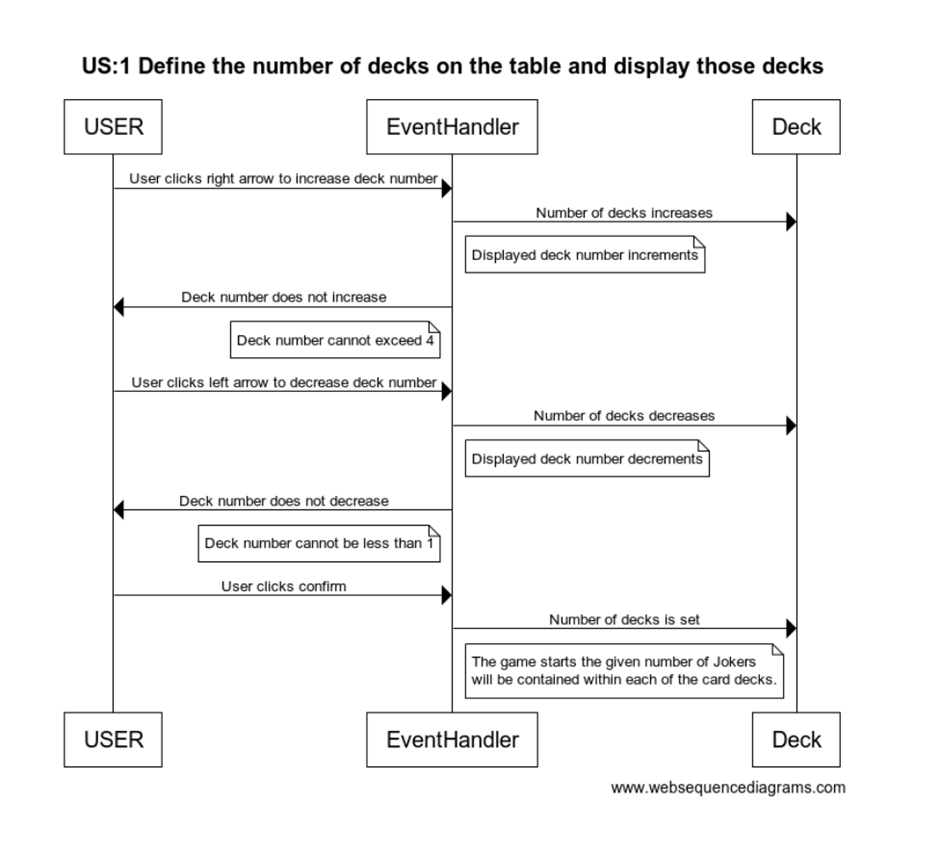
\includegraphics[width=0.95\linewidth]{assets/US1.png}
					\caption{US1 Sequence Diagram}
					\label{fig:us1-sequence}
				\end{figure}
				
				
				This sequence diagram outlines how a user sets the number of card decks for a game. The user can increase or decrease the deck count by clicking the right or left arrows, respectively. \\
				The event handler for click events updates and displays the new count but restricts the number to a minimum of 1 and a maximum of 4. Once the user clicks confirm, the event handler causes Deck to initialise the appropriate number of decks which are to be displayed in the game.
				
				\clearpage
				
				\begin{lstlisting}
					CLASS GameOptions
						INTEGER DeckCount <- 0
						
						METHOD GetDeckCount()
							RETURN DeckCount
						END METHOD
						
						METHOD ChangeDeckCount(Count)
							IF (DeckCount + Count) >= 1 AND (DeckCount + Count) <= 4 THEN
								DeckCount <- DeckCount + Count
							END IF
						END METHOD
					END CLASS
					
					CLASS Customization
						OBJECT OptionsInstance <- NEW GameOptions
						OBJECT IncreaseDeckCountButton <- NEW Button LABELED "+"
						OBJECT DecreaseDeckCountButton <- NEW Button LABELED "-"
						
						SET ACTION IncreaseDeckCountButton ON CLICK
							CALL OptionsInstance.ChangeDeckCount(1)
						END ACTION
						
						SET ACTION DecreaseDeckCountButton ON CLICK
							CALL OptionsInstance.ChangeDeckCount(-1)
						END ACTION
					END CLASS
				\end{lstlisting}
			
			\subsubsection*{US2: Number of Jokers per Deck}\label{subsubsec:us2-number-of-jokers-per-deck}
			
				\begin{figure}[H]
					\centering
					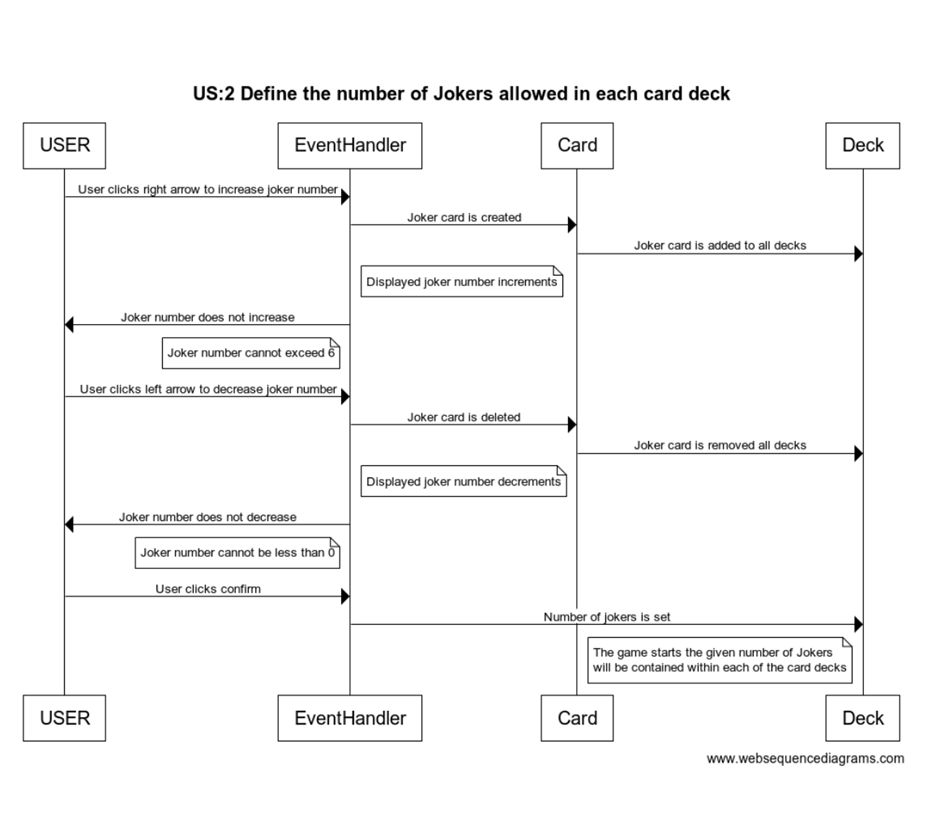
\includegraphics[width=0.8\linewidth]{assets/US2.png}
					\caption{US2 Sequence Diagram}
					\label{fig:us2-sequence}
				\end{figure}
				
				This sequence diagram details the process for configuring the number of Jokers to be included in each card deck before the game begins. The user can increase or decrease the deck count by clicking the right or left arrows, respectively. When increasing, a Joker Card is created and added to all Deck’s, while decreasing results in a Joker Card being removed. The system enforces limits, allowing a minimum of 0 and a maximum of 6 Jokers per Deck. Upon confirmation, the selected number of Jokers is set, and the game starts with the specified configuration applied to each Deck. \\\\
				
				\begin{lstlisting}
					// GameOptions Class
					CLASS GameOptions
						PRIVATE INTEGER JokerCount = 0
						
						PUBLIC METHOD GetJokerCount()
							RETURN JokerCount
						ENDMETHOD
						
						PUBLIC METHOD ChangeJokerCount(INTEGER Count)
							IF Count IS within acceptable joker range THEN
								JokerCount = JokerCount + Count
							ENDIF
						ENDMETHOD					
					ENDCLASS
					
					// Customization Class
					CLASS Customization
						Button increaseJokerCountButton = NEW Button("+")
						Button decreaseJokerCountButton = NEW Button("-")
					
						increaseJokerCountButton.SETONACTION(event -> GameOptions.ChangeJokerCount(1))
						decreaseJokerCountButton.SETONACTION(event -> GameOptions.ChangeJokerCount(-1))
					ENDCLASS
				\end{lstlisting}
			
			\subsubsection*{US3: Card Images}\label{subsubsec:us3-card-images}
			
				\begin{figure}[H]
					\centering
					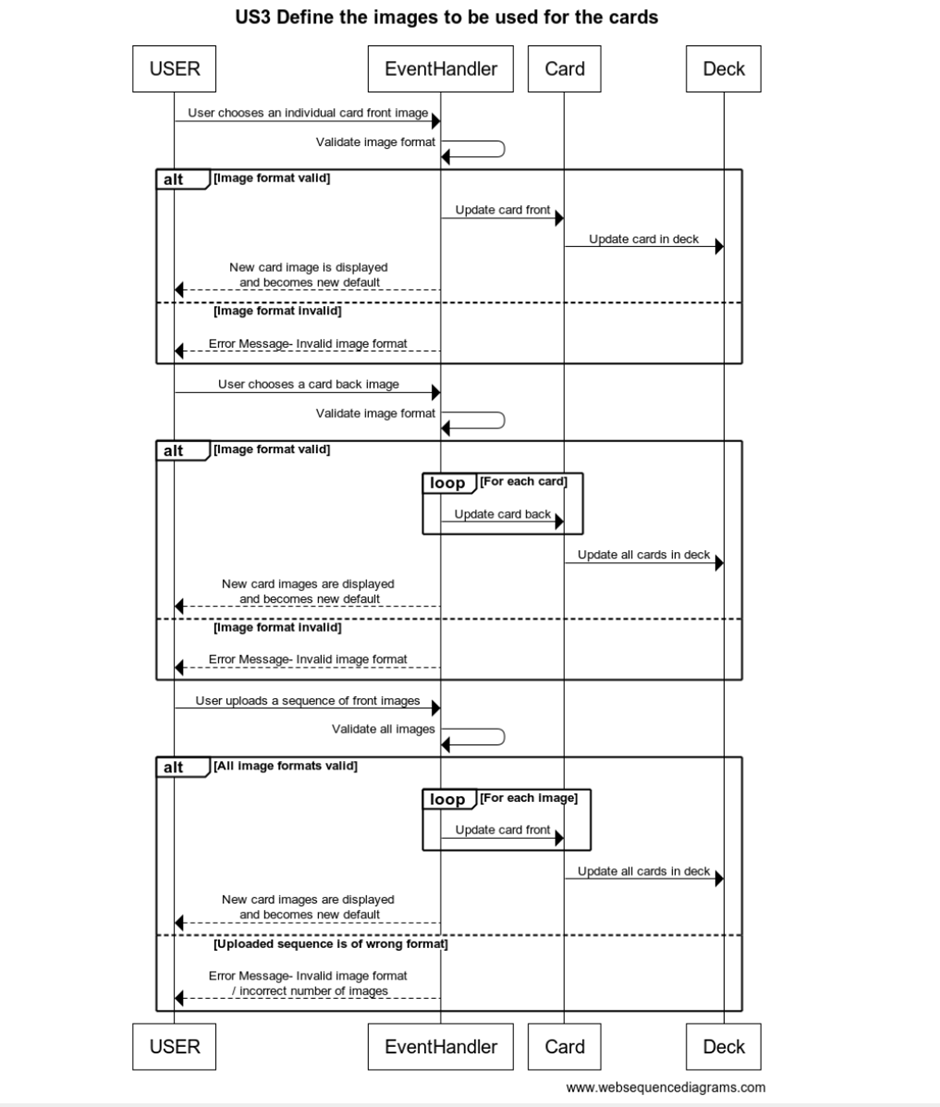
\includegraphics[width=0.9\linewidth]{assets/US3.png}
					\caption{US3 Sequence Diagram}
					\label{fig:us3-sequence}
				\end{figure}
				
				This sequence diagram describes the user interaction for customising card images used in the game. The user can select an individual front image, a back image, or upload a sequence of front images. For each action, the system first validates the image format. If valid, the selected image(s) are applied to the respective Cards, and the updated visuals are reflected in the Deck, becoming the new default. \\
				For individual images, the change is applied to the Card or all Cards as appropriate. When the user uploads a sequence of images, each Card front is updated accordingly. If any image format is invalid or the sequence is incorrect, the event handler that got the images displays an appropriate error message, preventing the update.
				
				\begin{lstlisting}
					BEGIN selectCardImage
						CHECK image has not been selected
						CREATE a fileChooser title to "tap to change card image"
						
						DEFINE fileFilters for images (JPG, PGN, etc...)
						APPLY fileFilters to FileChooser
						
						OPEN fileChooser dialog and STORE selected files
						IF file is NOT selected THEN
							EXIT function
						ENDIF
						
						CONVERT selected file to an Image object
						
						CREATE a CardImage using image
						CREATE a Card with the CardImage
						
						APPLY FrontCard to ALL Cards
						
						IF singleCard is selected to have a new CardImage
							FOR singleCard:
								SELECT new image
								APPLY new image to single Card
							UPDATE deck
						ENDIF
					END selectCardImage
					
				\end{lstlisting}
				
			\pagebreak
			
			\subsection*{US4: Customize Background}\label{subsubsec:us4-Customize-Background}
			
				\begin{figure}[ht]
					\centering
					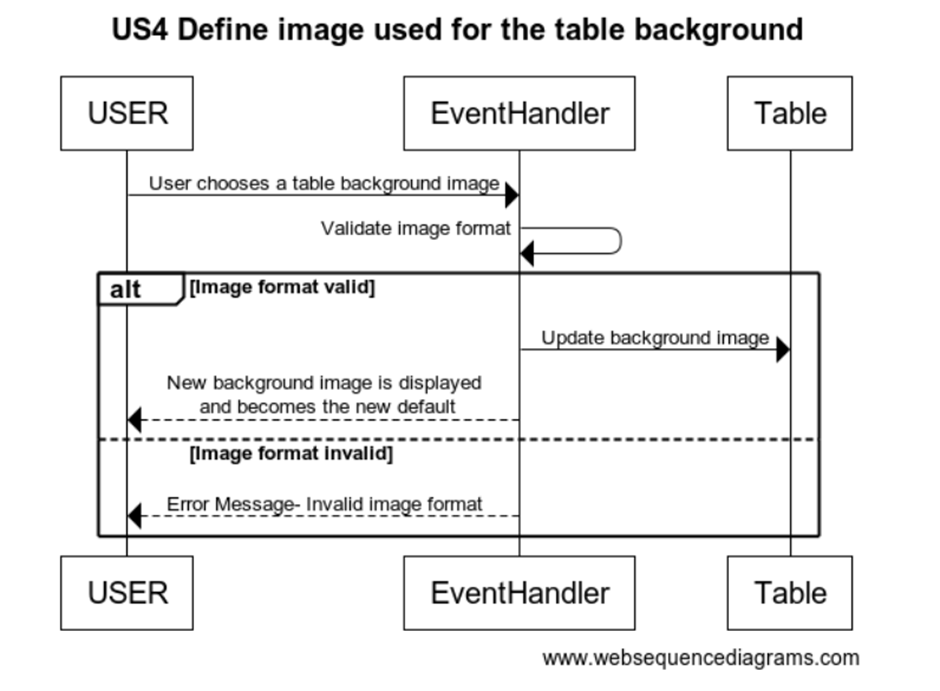
\includegraphics[width=\linewidth]{assets/US4.png}
					\caption{US5 Sequence Diagram}
					\label{fig:us4-sequence}
				\end{figure}
				
				This sequence diagram outlines the process for setting a custom table background image. \\
				When the user selects an image, the event handler that was used to select it validates its format. If the image is valid, the background is updated on the table, and the new image is displayed as the default. \\
				If the image format is invalid, the event handler notifies the user with an appropriate error message, and the background remains unchanged. \\\\
				
				\begin{lstlisting}
					BEGIN SelectAndSetBackgroundImage
						CREATE a FileChooser object
						SET fileChooser title to "Select an Image"
						
						DEFINE fileFilters for images (JPG, PNG, etc.)
						APPLY fileFilters to fileChooser
						
						OPEN fileChooser dialog and STORE selected file
						IF file is NOT selected THEN
							EXIT function
						ENDIF
						
						CONVERT selected file to an Image object
						CREATE a BackgroundImage using the Image
						CREATE a Background with the BackgroundImage
						
						APPLY Background to the thumbnail/board background
					END SelectAndSetBackgroundImage
				\end{lstlisting}
			
			\subsubsection*{US5: Shuffling Decks}\label{subsubsec:us5-shuffling-decks}
			
				\begin{figure}[H]
					\centering
					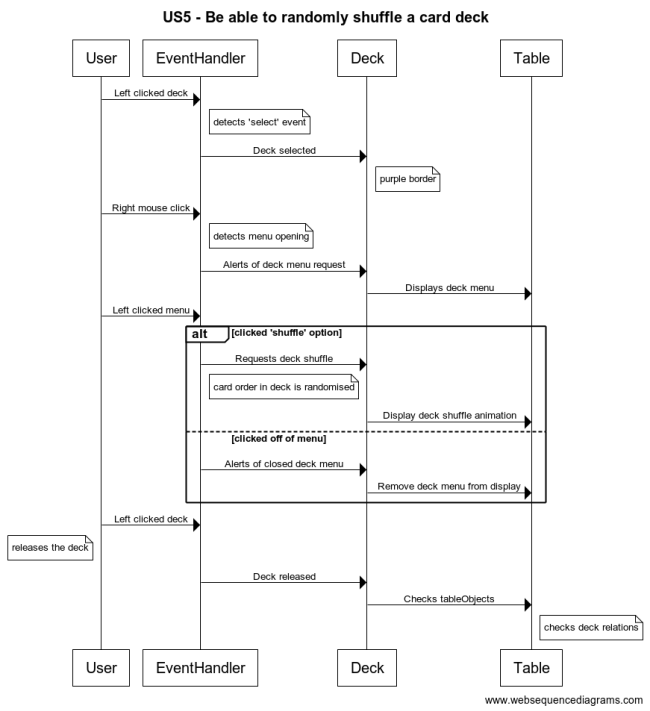
\includegraphics[width=0.95\linewidth]{assets/US5.png}
					\caption{US5 Sequence Diagram}
					\label{fig:us5-sequence}
				\end{figure}
				
				The sequence diagram above shows how a user randomly shuffles a selected card deck. When the user clicks on the deck, the system detects this as a selection event, highlighting the deck with a purple border to indicate its new state. A right-click triggers a menu-opening event, resulting in the deck menu being displayed. If the user selects the shuffle option, the system randomises the order of the cards within the deck and triggers a shuffle animation. If the user instead decides to click away from the menu, the system closes the menu, removing it from view. Finally, when the user releases the deck, the system marks the deck as released, and the Table component checks for any relational updates between the deck and other table objects.
				
				\begin{lstlisting}
					Shuffle(deck)
						IF deck IS OF TYPE Deck THEN
							Randomly shuffle the cards in deck
							Update the deck with the shuffled order
							Play shuffle animation
						END IF
					END
				\end{lstlisting}
			
			\subsubsection*{US6: Move a Card}\label{subsubsec:us6-move-a-card}
			
				\begin{figure}[ht]
					\centering
					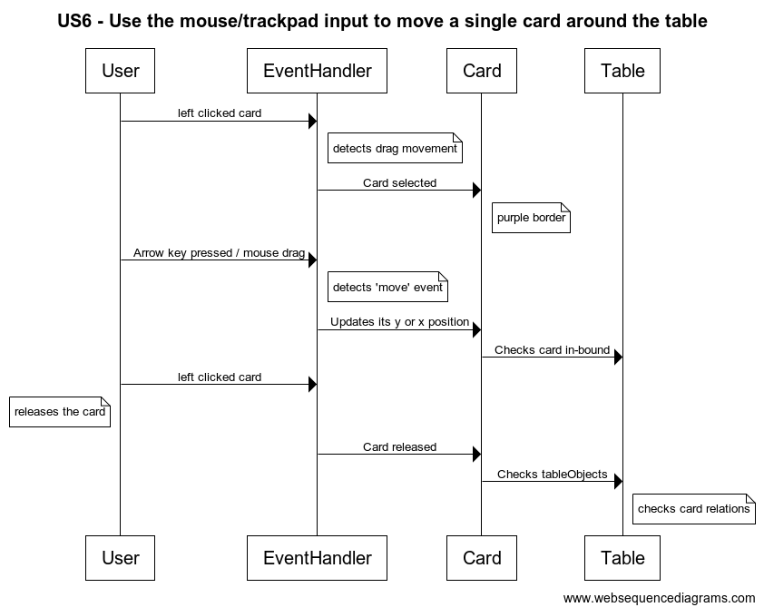
\includegraphics[width=\linewidth]{assets/US6.png}
					\caption{US6 Sequence Diagram}
					\label{fig:us6-sequence}
				\end{figure}
				
				The sequence diagram above shows how a user moves a single card across the table using either arrow keys or drag-and-drop input. When the system detects the user’s initial card click, the selected card is visually highlighted with a purple border. As the user moves the card using input controls, the system registers this as a movement event and updates the card’s x or y position accordingly. The card then checks whether it remains within the table bounds, and once the user releases the card, the system finalises the action and checks for any interactions between the card and other table objects.
				
				\begin{lstlisting}
					selectedCard = NULL
					offsetX = 0
					offsetY = 0
					
					// Event handler for mouse press (when the user clicks on a card)
					ON MousePressed(Event):
						IF mouse click is on a card:
							selectedCard = card clicked
							
							// Record the position of the mouse relative to the card's position
							offsetX = mouse X position - selectedCards X position
							offsetY = mouse Y position - selectedCards Y position
						END IF
					END MousePressed
					
					// Event handler for mouse drag (when the user drags the card)
					ON MouseDragged(Event):
						IF selectedCard is NOT NULL:
							// Update the position of the selected card to follow the mouse
							newX = mouse X position - offsetX
							newY = mouse Y position - offsetY
							
							// Move the selected card to the new position
							selectedCards X position = newX
							selectedCards Y position = newY
						END IF
					END MouseDragged
					
					// Event handler for mouse release (when the user releases the card)
					ON MouseReleased(Event):
						// Once the card is released, stop tracking the card
						selectedCard = NULL
					END MouseReleased
				\end{lstlisting}
				
				1. Card Selection:
				The user selects a card using a mouse or keyboard shortcut. \\
				The selected card’s current position and orientation (face-up or face-down) are stored.
				
				2. Card Movement:
				The user drags the card with a mouse or uses keyboard input (e.g., arrow keys) to move the card. \\
				As the user moves the card, its position is updated dynamically. \\
				The position is checked to ensure that it stays within the bounds of the table (no off-screen movement).
				
				3. Card Placement:
				When the user stops dragging or releases the mouse (or presses a key), the card is finalized in its new position. \\
				If the new position overlaps with another card, the system resolves the overlap by stacking the cards according to their layering rules (e.g., top card or underneath). \\
				The card's orientation is maintained (it stays face-up or face-down as it was when picked up).
				The card is displayed in the new position.
			
			\subsubsection*{US7: Reposition a Card in a Group}\label{subsubsec:us7-reposition-a-card-in-a-group}
			
				\begin{figure}[H]
					\centering
					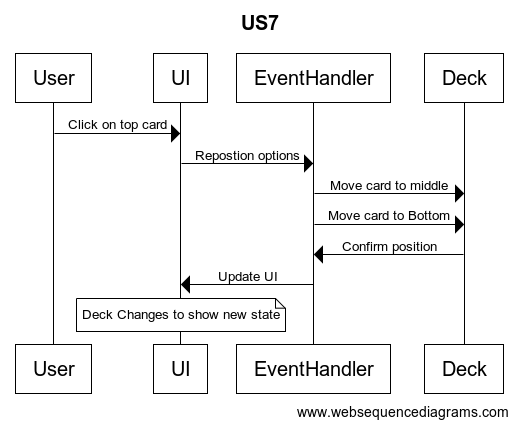
\includegraphics[width=0.6\linewidth]{assets/US7.png}
					\caption{US7 Sequence Diagram}
					\label{fig:us7-sequence}
				\end{figure}
				
				
				In this interaction, the system allows a user to reposition a card within a group of cards to ensure smooth and flexible gameplay. \\
				The user can select the top card from a group and move it to a different position within that same group.  \\
				The card can be placed at the bottom or somewhere else in the group through a popup option interaction activated by the right click of the mouse. \\
				When the user selects the card, the UI communicates with the group using the click event handler, which handles the repositioning and updates the group accordingly. \\
				The UI provides visual feedback while the repositioning is happening and again when it is complete, confirming the card has been moved successfully.
				
				\begin{lstlisting}
					// Function To Reposition The Top Card Within A Selected Deck
					FUNCTION
						// Remove topCard from selectedDeck so that it can then be moved to its updated position
						DEFINE topCard <- selectedDeck[0]
						
						IF moveToBottom IS TRUE THEN
							APPEND topCard TO top OF selectedDeck
						ELSE
							// Randomly select a new index possition for the topCard somewhere in the deck
							randomIndex <- RANDOM GENERATED INTEGER FROM 1 TO length of selectedDeck
							INSERT topCard AT randomIndex IN selectedDeck
						ENDIF
						
						RETURN selectedDeck
					END FUNCTION
				\end{lstlisting}
			
			\subsubsection*{US8:Move Multiple Cards}\label{subsubsec:us8-move-multiple-cards}
			
				\begin{figure}[H]
					\begin{center}
						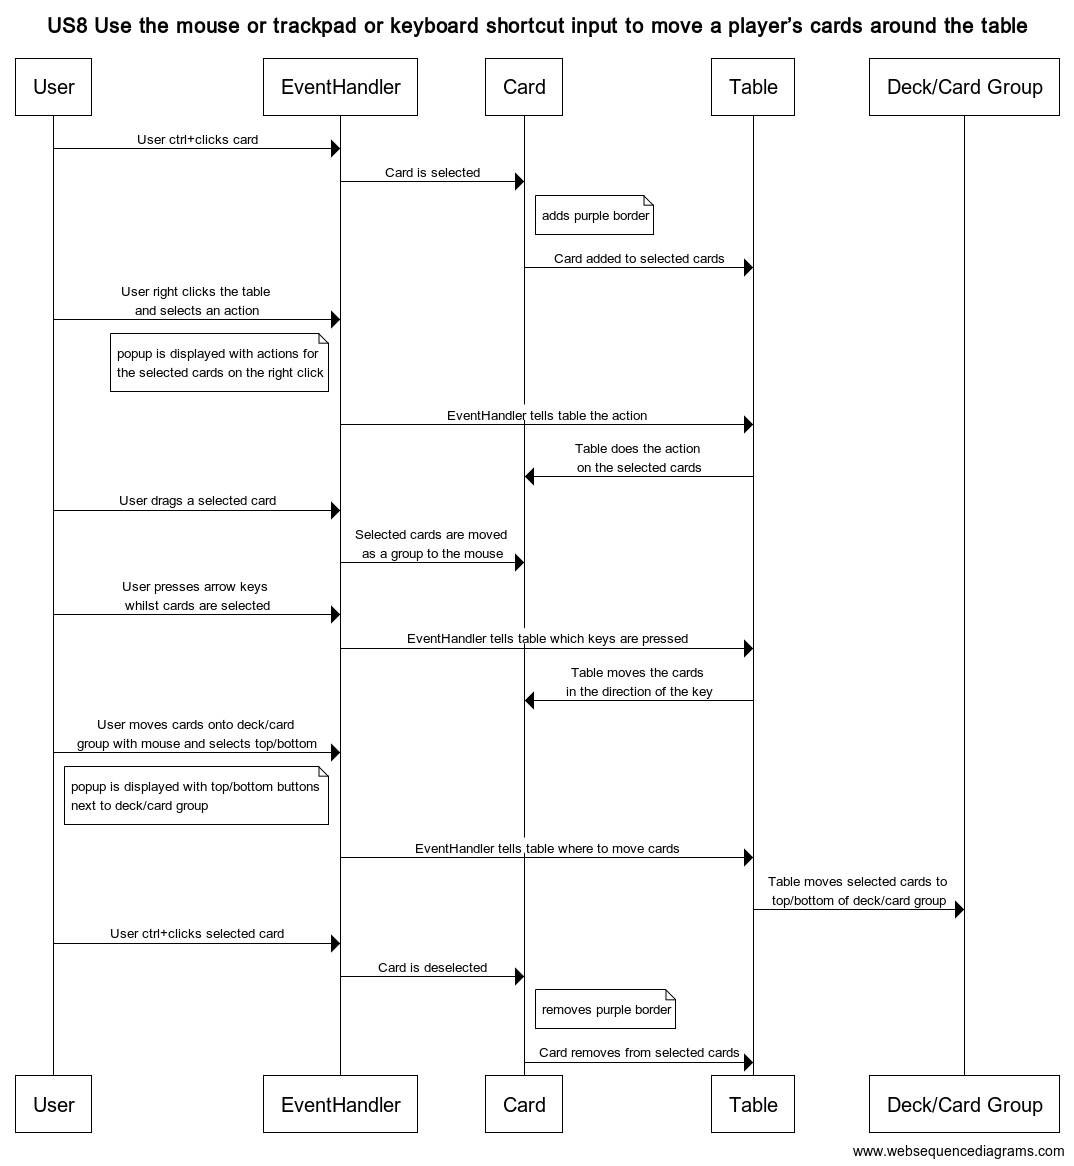
\includegraphics[width=\linewidth]{assets/US8.png}
						\caption{US8 Sequence Diagram}
						\label{fig:us8-sequence}
					\end{center}
				\end{figure}
				
				\textbf{Step 1: User Selects a Subset of Cards} \\
				WAIT for input: The program waits for the user to select cards, either through mouse clicks or keyboard shortcuts. \\
				IF cards selected THEN: \\
				Once the user selects cards, the program: \\
				- SELECT a subset of cards (this could involve clicking or dragging multiple cards). \\
				- REVEAL faces of selected cards (if the cards are face-down, they are flipped to face-up for easier decision-making). \\
				- STORE selected cards in a list - The program keeps track of which cards are selected for further manipulation. \\
				
				\textbf{Step 2: User Moves the Selected Cards} \\
				WAIT for drag or keyboard input: The program waits for the user to start moving the cards, either by dragging them with the mouse or using keyboard keys. \\
				IF dragging or keyboard movement starts THEN: \\
				- DISPLAY visual feedback: The program highlights or outlines the cards being moved to give feedback to the user. \\
				- STORE initial position: The starting position and orientation of the cards are saved to keep track of where they were originally placed. \\ \\
				WHILE dragging or moving with keyboard: \\
				As long as the user continues to drag or use keyboard input: \\
				For each card: \\
				- If the user presses arrow keys or WASD, the cards are moved in the corresponding direction. \\
				- If the user is dragging with the mouse, the cards' positions are updated based on the mouse's movement. \\
				- Ensure cards stay on the table: The program checks that cards do not move off the visible table area. If they do, their position is adjusted to stay within bounds. \\
				- Display updated position: The visual feedback is updated to show the new location of the cards. \\
				
				\textbf{Step 3: User Drops the Cards} \\
				WAIT for mouse release or keyboard stop: \\
				The program waits until the user releases the mouse or stops using keyboard input. \\
				IF release THEN: \\
				The program checks where the cards were dropped: \\
				- On a deck: If the cards are dropped on a deck, they are placed on top of it. \\
				- In an empty space: If the cards are dropped in an empty space, they are placed there. \\
				Ensure cards' orientation remains intact: After being dropped, the cards' orientations (face-up or face-down) are restored to their original state. \\
				Display final feedback: The program provides visual feedback that the operation is complete, such as fading out highlights or animating the cards being placed. \\
				
				\textbf{Step 4: Reset UI} \\
				Remove feedback: The program removes any visual feedback (like highlights or outlines) used during the move. \\
				Reset the UI: It resets the user interface, including deselecting any selected cards - Update card positions: The final positions of the cards are updated and stacked appropriately.
				
				\clearpage
				
				\begin{lstlisting}
					START
						// Step 1: User selects a subset of cards
						WAIT for input to select cards
						IF cards selected THEN
							SELECT subset of cards
							REVEAL faces of selected cards
							STORE selected cards in a list
						END IF 
						
						// Step 2: User moves the selected cards
						WAIT for drag or keyboard input
						IF user starts dragging or moves with keyboard THEN
							DISPLAY visual feedback
							STORE initial position and orientation
						
							WHILE dragging or moving with keyboard DO
								FOR each card DO
									IF arrow/WASD keys THEN MOVE card in direction
									ELSE IF mouse drag THEN UPDATE position with offset
								END FOR
							
								FOR each card DO
									IF position off table THEN ADJUST position
								END FOR
							
								DISPLAY updated position
							END WHILE
						END IF
						
						// Step 3: User drops cards
						WAIT for mouse release or keyboard stop
						IF release THEN
							IF dropped on deck THEN PLACE on deck
							ELSE IF dropped in empty space THEN PLACE in space
					
							FOR each card DO
								SET card orientation to original
							END FOR
					
							DISPLAY final feedback
						END IF
						
						// Step 4: Reset UI
						REMOVE feedback
						RESET UI (deselect cards, reset highlights)
						UPDATE card positions
					END
				\end{lstlisting}
				
				
				\clearpage
			
			\subsubsection*{US9: Flip a Card}\label{subsubsec:us9-flip-a-card}
			
				\begin{figure}[H]
					\centering
					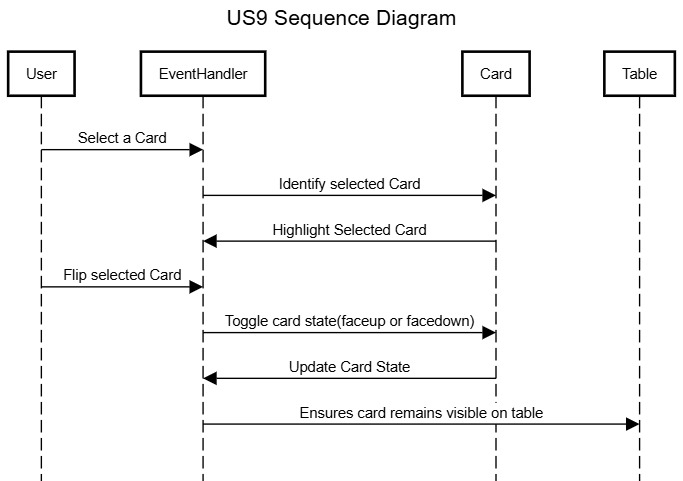
\includegraphics[width=0.75\linewidth]{assets/US9.jpg}
					\caption{US9 Sequence Diagram}
					\label{fig:us9-sequence}
				\end{figure}
				
				The sequence diagram above shows how a user selects and flips a card during a game. The event handler for the flip button processes the selection, identifies the card by hovering over it, and highlights it. When the user flips the card, the flip button event handler updates its state via the Card's class. A flipped card is then displayed on the table.
			
			\subsubsection*{US10: Flip Multiple Cards}\label{subsubsec:us10-flip-multiple-cards}
			
				\begin{figure}[H]
					\centering
					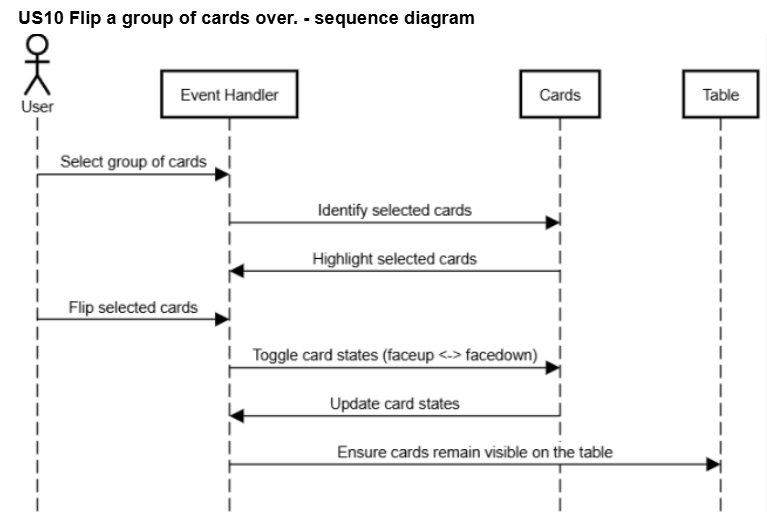
\includegraphics[width=0.85\linewidth]{assets/US10.png}
					\caption{US10 Sequence Diagram}
					\label{fig:us10-sequence}
				\end{figure}
				
				The sequence diagram above shows how a user selects and flips cards during a game. The event handler for the flip button processes the selection, identifies the cards by hovering over them, and highlights them. When the user flips the cards, the flip button event handler updates their states via the Card's class. The flipped cards are then displayed on the table.
			
			\subsubsection*{US11: Reveal Cards}\label{subsubsec:us10-reveal-cards}
			
				\begin{figure}[H]
					\centering			
					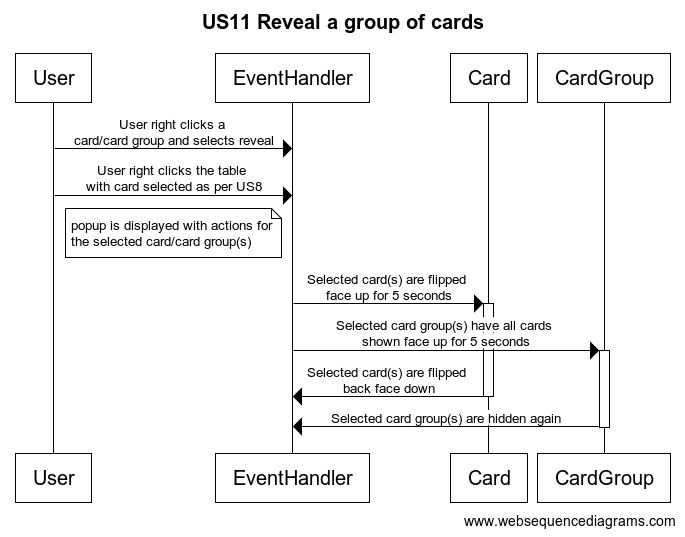
\includegraphics[width=1.0\linewidth]{assets/US11.jpg}
					\caption{US11 Sequence Diagram}
					\label{fig:us11-sequence}
				\end{figure}
				
				The US11 Sequence Diagram outlines the process for revealing a Card or Card group through the user interface. The user initiates this by right clicking a Card or group and selecting "reveal" from the popup menu, triggering the button's event handler to flip the selected Card(s) face up for 5 seconds before flipping them back down. If a group of cards is selected, all Cards within it are revealed simultaneously. The Card entities handle the visual state changes.
				
				\clearpage
			
			\subsubsection*{Pseudocode for US9, US10, US11}
			
				\begin{lstlisting}
					// have a data structure which keeps track of what objects have been selected
					DEFINE selected = cards
					
					// if left click action detected, check if clicked object can be added to selected list
					IF action == leftClick THEN
						// if yes then append to data structure
						IF selected.type == selectedObj THEN
							selected[+1] = selectedObj
						ENDIF
						
					// if right click action detected, depending on the type of objects selected, either open single card or group of cards menu
					ELSEIF action == rightClick THEN
						IF selected.type == single THEN
							// depending on button clicked, act appropriately on the selected case
							SWITCH singleMenu
								CASE flip:
									// for loop goes through all selected cards and reverses 'cardFacing' bool
									selected.flip()
								CASE reveal:
									selected.flip()
									delay(5s)
									selected.flip()
								CASE rotate:
									// Rotate
								CASE default:
									leaveMenu
							ENDSWITCH
						ELSE THEN
							// depending on button clicked, act appropriately on the selected case
							SWITCH groupMenu
								CASE flip: 
									selected.flip()
								CASE shuffle:
									// Shuffle
								CASE reveal:
									selected.flipAll()
									delay(5s)
									selected.flipAll()
								CASE rotate:
									// Rotate
								CASE default:
									leaveMenu
							ENDSWITCH
						ENDIF
					ENDIF
				\end{lstlisting}
				
				\clearpage
			
			\subsubsection*{US12: Save Dealing Layout}\label{subsubsec:us12-save-dealing-layout}
			
				\begin{figure}[ht]
					\centering
					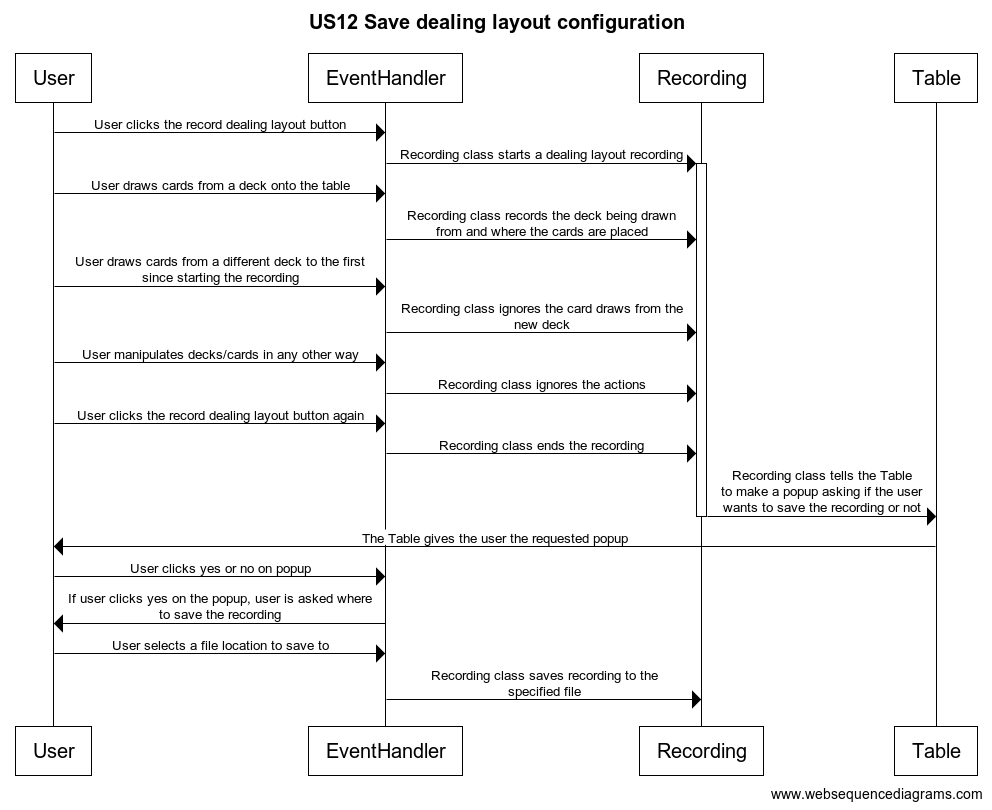
\includegraphics[width=\linewidth]{assets/US12.png}
					\caption{US12 Sequence Diagram}
					\label{fig:us12-sequence}
				\end{figure}
				
				The sequence diagram above shows how a user records and saves a dealing layout configuration. When the user clicks the record layout button, the system begins tracking card placements from the selected deck. As the user draws cards from the selected deck onto the table, the recording class captures each placement. If the user performs unrelated actions, they are ignored by the system. When the user clicks the record button again, the recording stops and a popup appears asking whether to save the layout. If the user confirms, they are prompted to choose a save location, and the recording is saved.
				
				\vfill
				
				\begin{lstlisting}
					// When dealing layout recording button is pressed
					createNewCardActionRecordingThread()
					
					// After any action is taken in game
					GameAction gameAction = createGameActionFromEvent()
					actionQueue.add(gameAction)
					
					// To end a dealing layout recording (same button as starting one)
					GameAction endAction = createGameActionDealingEndSignal(shouldSave)
					actionQueue.add(endAction)
					
					// In the recording thread
					recording = true
					WHILE (recording)
						// thread safe, waits for update
						action = getActionQueue().take()
					
						// If it should end, end
						IF (isEndSignal(action))
							IF (action.shouldSave())
								saveRecordingQueueToFile()
							ENDIF
							recording = false
						ENDIF
						
						// If the action is something that works incrementally like rotating, it merges it with the
						// previous action so you dont have an action for each degree of rotation of the same card
						action = checkMergeAction(action)
						
						// If only recording a dealing layout, ignore irrelevant actions
						IF (!isCardAction(action) AND !isRecordingAll)
							continue;
						ENDIF
						
						// Push it to a queue to be saved
						recordingQueue.add(action)
					NEXT
				\end{lstlisting}
				
				\clearpage
			
			\subsubsection*{US13: Deal Cards From Layout}\label{subsubsec:us13-deal-cards-from-a-layout}
			
				\begin{figure}[H]
					\centering
					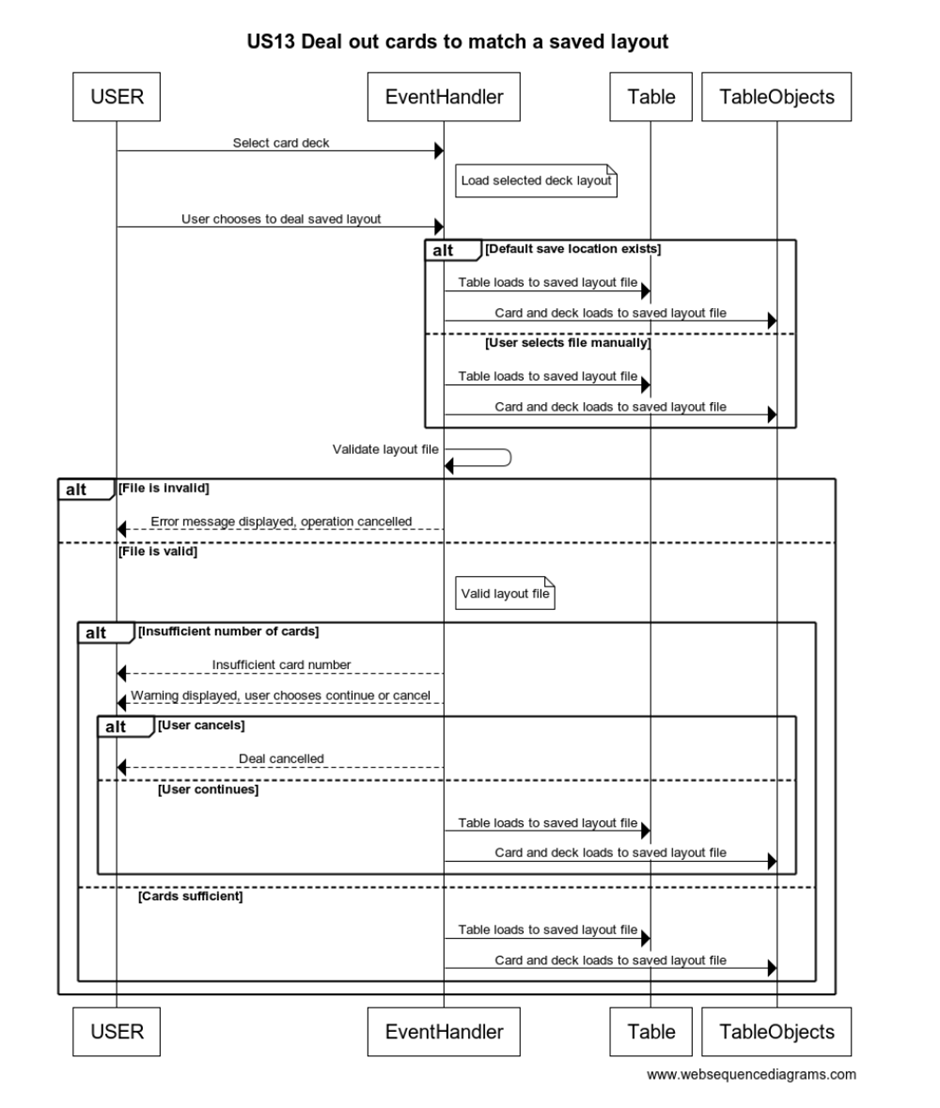
\includegraphics[width=\linewidth]{assets/US13.png}
					\caption{US13 Sequence Diagram}
					\label{fig:us13-sequence}
				\end{figure}
				
				This sequence diagram describes the process of dealing cards to match a previously saved table layout. The user first selects a card deck, triggering the deck's event handler to load the corresponding layout. When the user chooses to deal the saved layout, the system attempts to load the layout either from a default location or a user-selected file. The layout file is then validated. If the file is invalid, an error message is shown, and the operation is cancelled. If valid, the system checks whether there are enough cards to complete the layout. If not, the user is warned and given the option to proceed or cancel. If the user proceeds, or if the card count is sufficient from the start, the table and associated cards are dealt based on the saved configuration.
				
				\begin{lstlisting}
					deck=card_deck
					
					If the file chosen exists then get dealing layout file
					else display an error
					
					If the number of instructions for dealing is more then the size of deck chosen then issue a warning
					
					Once conditions are checked and file is validated,
					
						Until instructions are available, parse the file instructions and perform the action
					
						Print message specifying completion
				\end{lstlisting}
				
			\subsubsection*{US14: Rotate Cards}\label{subsubsec:us14-rotate-cards}
			
				\begin{figure}[H]
					\centering
					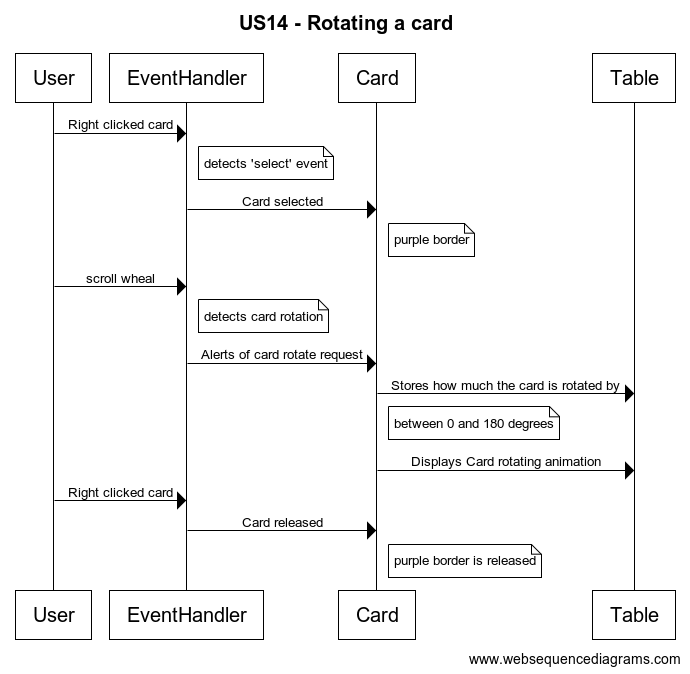
\includegraphics[width=0.9\linewidth]{assets/US14.png}
					\caption{US14 Sequence Diagram}
					\label{fig:us14-sequence}
				\end{figure}
				
				The sequence diagram above shows how a user rotates a selected card. When the user clicks on a card, the system recognises this interaction as an event. This prompts the system to create a rotate transition, which is configured with key parameters like duration, rotation axis, and angle. Once the transition is set up, it’s played to animate the card flipping along the Y-axis. After the animation completes, the card's rotation is reset, ensuring it's ready for future interactions.
				
				\begin{lstlisting}
					BEGIN Rotate
						SET card to be faceDown
						
						IF RotateOption is available:
							CREATE rotateTransition
							CREATE ImageChangeTransition
							CREATE ParallelTransition using rotateTransition AND ImageChangeTransition
							
							APPLY ParallelTransition ON cards
							
							CREATE 5-second delay
							
							CREATE SequentialTransiton using ParallelTransition AND delay AND ParallelTransition
							
							PLAY SequentialTransiton
						ENDIF
						
						SET Card to be returned faceDown
					END Rotate
				\end{lstlisting}
				
				\clearpage
			
			\subsubsection*{US15: Record Games}\label{subsubsec:us15-record-games}
			
				\begin{figure}[H]
					\centering
					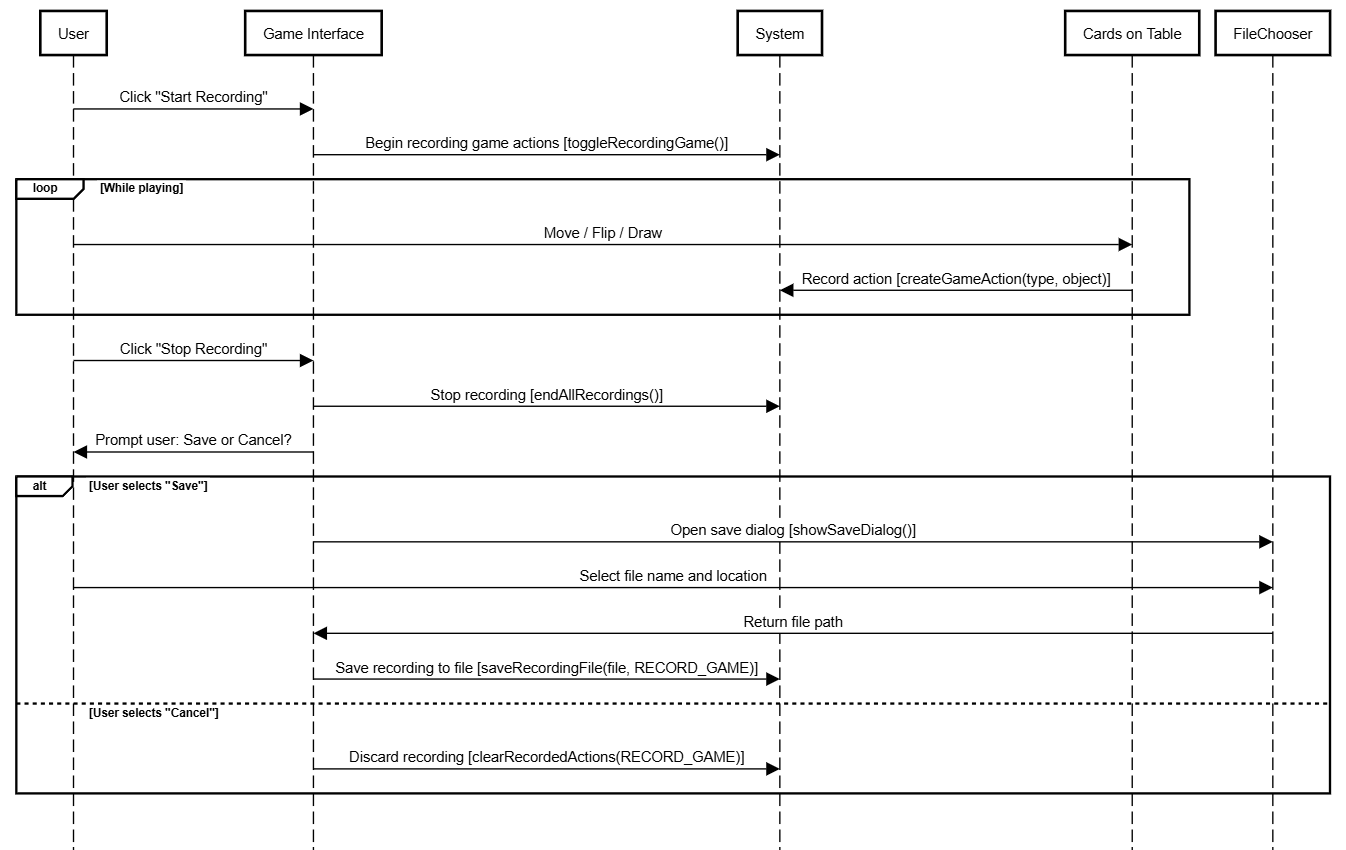
\includegraphics[width=1\linewidth]{assets/US15.png}
					\caption{US15 Sequence Diagram}
					\label{fig:us15-sequence}
				\end{figure}
				
				The sequence diagram outlines the interactions involved in recording a game session. It begins when the user selects the option to start recording from the game interface, typically by clicking a “Start Recording” button. This triggers the system to enable recording mode via a method like toggleRecordingGame(). From that moment onward, all gameplay actions, such as moving cards, flipping them, or drawing from a deck, are captured. Each time the user performs an action, the associated card or table object notifies the system, which creates and stores a GameAction using createGameAction(type, object). This loop continues until the user explicitly stops the recording by clicking “Stop Recording”. At that point, the system prompts the user with a dialog box asking whether to save or discard the recording. If the user chooses to save, a FileChooser dialog is opened (showSaveDialog()), allowing the user to choose a filename and location for the recording. The system then writes the list of recorded actions to the selected file using saveRecordingFile(file, RECORD\_GAME). Alternatively, if the user cancels, the system discards the recorded actions using clearRecordedActions(RECORD\_GAME), and nothing is saved. This flow ensures that users can preserve game sessions for future playback, or abandon them entirely if no longer needed.
				
				\vfill
				
				\begin{lstlisting}
					// When recording button is pressed
					createNewRecordingThread()
					
					// After any action is taken in game
					GameAction gameAction = createGameActionFromEvent()
					actionQueue.add(gameAction)
					
					// To end a dealing layout recording (same button as starting one)
					GameAction endAction = createGameActionEndSignal(shouldSave)
					actionQueue.add(endAction)
					
					// In the recording thread
					recording = true
					WHILE (recording)
						// thread safe, waits for update
						action = getActionQueue().take()
						
						// If it should end, end
						IF (isEndSignal(action))
							IF (action.shouldSave())
								saveRecordingQueueToFile()
							ENDIF
							recording = false
						ENDIF
						
						// If the action is something that works incrementally like rotating, it merges it with the
						// previous action so you dont have an action for each degree of rotation of the same card
						action = checkMergeAction(action)
						
						// If only recording a dealing layout, ignore irrelevant actions
						IF (!isCardAction(action) AND !isRecordingAll)
							continue;
						ENDIF
						
						// Push it to a queue to be saved
						recordingQueue.add(action)
					NEXT
				\end{lstlisting}
				
				\clearpage
			
			\subsubsection*{US16: Replay Games}\label{subsubsec:us16-replay-games}
			
				\begin{figure}[H]
					\centering
					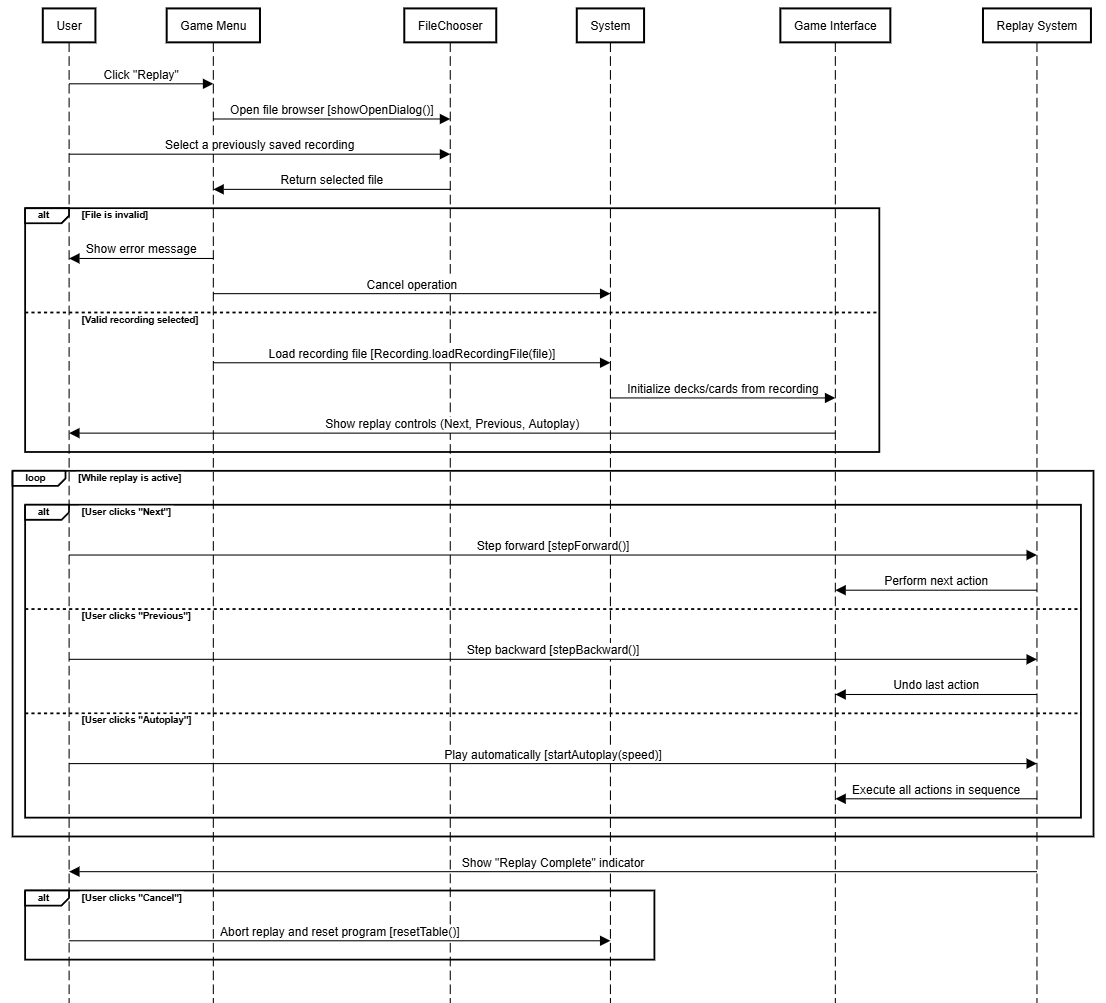
\includegraphics[width=1\linewidth]{assets/US16.png}
					\caption{US16 Sequence Diagram}
					\label{fig:us16-sequence}
				\end{figure}
			
				The sequence diagram illustrates how the user interacts with the system to replay a previously recorded game. The process begins when the user selects the “Replay” option from the game’s main menu, which prompts the system to open a file browser dialog (via a FileChooser) where the user can navigate to and select a previously saved recording. If the file is invalid, for example if it’s not a proper recording or is corrupted, the system displays an error message and cancels the operation. However, if a valid file is selected, the system loads the recording using Recording.loadRecordingFile(file) and initializes the game interface, setting up the decks and cards as they were when the recording began. Replay controls are then displayed, allowing the user to step through the game manually or start automatic playback. The user can press “Next” to step forward one move at a time, or “Previous” to step backward, with each move executed or undone through the game interface. Alternatively, the user may choose “Autoplay,” which plays the entire recording at a predefined speed (startAutoplay(speed)), automatically executing each move. Once the replay is complete, the system displays a visual indicator to notify the user. At any point during the replay, the user can cancel the operation, which stops the playback and resets the game state using resetTable().
				
				\vfill
				
				\begin{lstlisting}
					deck = card_deck
					IF recording file exists
						get game recording layout file;
					ELSE display error
					
					//play whole game recording
					WHILE recorded action available
						parse recorded action
						follow instruction;
					NEXT
					
					display done message
				\end{lstlisting}
			
			\subsubsection*{US17: Snap to Grid}\label{subsubsec:us17-snap-to-grid}
			
				\begin{figure}[ht]
					\centering
					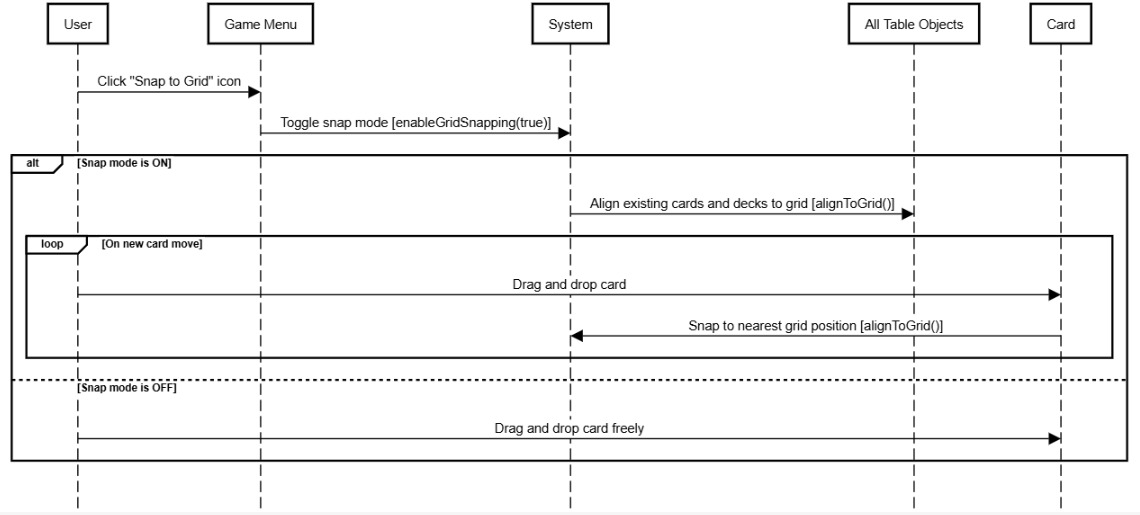
\includegraphics[width=1\linewidth]{assets/US17.jpg}
					\caption{US17 Sequence Diagram}
					\label{fig:us17-sequence}
				\end{figure}
				
				The sequence diagram for US17 includes both the activation of snap-to-grid mode and the alignment of all current cards and decks. When the user clicks the “Snap to Grid” icon from the game menu, the system toggles a flag to enable snap mode e.g., enableGridSnapping(true). The system scans the table and calls alignToGrid() on all currently placed objects, repositioning them to the nearest grid-aligned coordinates. This ensures the entire table appears structured when the feature is activated. From that point, whenever the user drags or drops a card, the system intercepts the movement and snaps the card to the nearest grid cell. If the user disables snap mode, the system stops intercepting movement and cards can be placed freely again. \\\\\\
				
				\begin{lstlisting}
					FUNCTION snapToGrid(card)
						x = getCardX(card)
						y = getCardY(card)
						rotation = getCardRotation(card)
						
						nearestX = findClosestGridX(x)
						nearestY = findClosestGridY(y)
						
						IF rotation >= -45 AND rotation <= 45 THEN
							newRotation = 90
						ELSE
							newRotation = 0
						ENDIF
						
						updateCardPosition(card, nearestGridX, nearestGridY)
						updateCardRotation(card, newRotation)
					END FUNCTION
					
					// On enabling Snap To Grid
					FOR EACH card IN Cards
						snapToGrid(card)
					ENDFOR
					drawGridLines(cardWidth)
					
					// Snap cards to grid while the feature is enabled
					WHILE snapToGridIsEnabled
						IF cardHasMoved THEN
							snapToGrid(movedCard)
						ENDIF
					ENDWHILE
					
					// On disabling Snap To Grid
					removeGridLines()
				\end{lstlisting}
			
			\subsubsection*{US18: Sound Effects}\label{subsubsec:us18-sound-effects}
			
				\begin{figure}[ht]
					\centering
					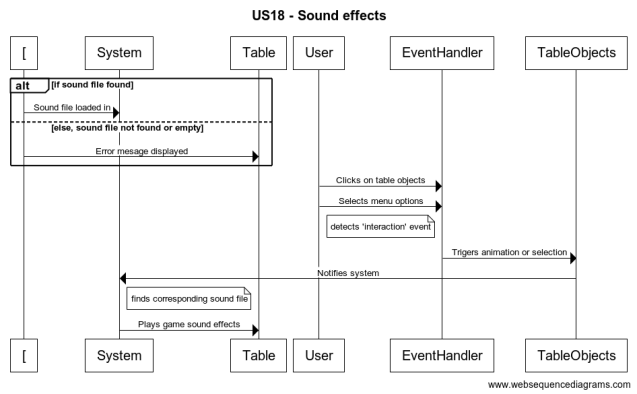
\includegraphics[width=1\linewidth]{assets/US18.png}
					\caption{US18 Sequence Diagram}
					\label{fig:us18-sequence}
				\end{figure}
				
				The sequence diagram above illustrates how sound effects are handled when a user interacts with table objects. At startup, the system attempts to load a sound file; if the file is found, it is loaded into memory, otherwise, the table displays an error message. When the user clicks on any table elements or selects options from their menu, the event is detected as an interaction, and the appropriate button's event handler checks if it triggers an animation or selection, some kind of action, so that it can then know if it should notify the system, which searches for and plays the corresponding sound effect to match the interaction.
				
				\begin{lstlisting}
					BEGIN PlaySoundOnCardClick
						LOAD sound file into an AudioClip object
						
						IF sound file fails to load THEN
							DISPLAY error message
						EXIT function
					END PlaySoundOnCardClick
					
					DEFINE action to be done on card click
					CONFIGURE card object so that when clicked, it plays the sound effect
				\end{lstlisting}
				
				\clearpage
		
		\subsection{State diagram}\label{subsec:state-diagram}
		
			\begin{figure}[H]
				\centering
				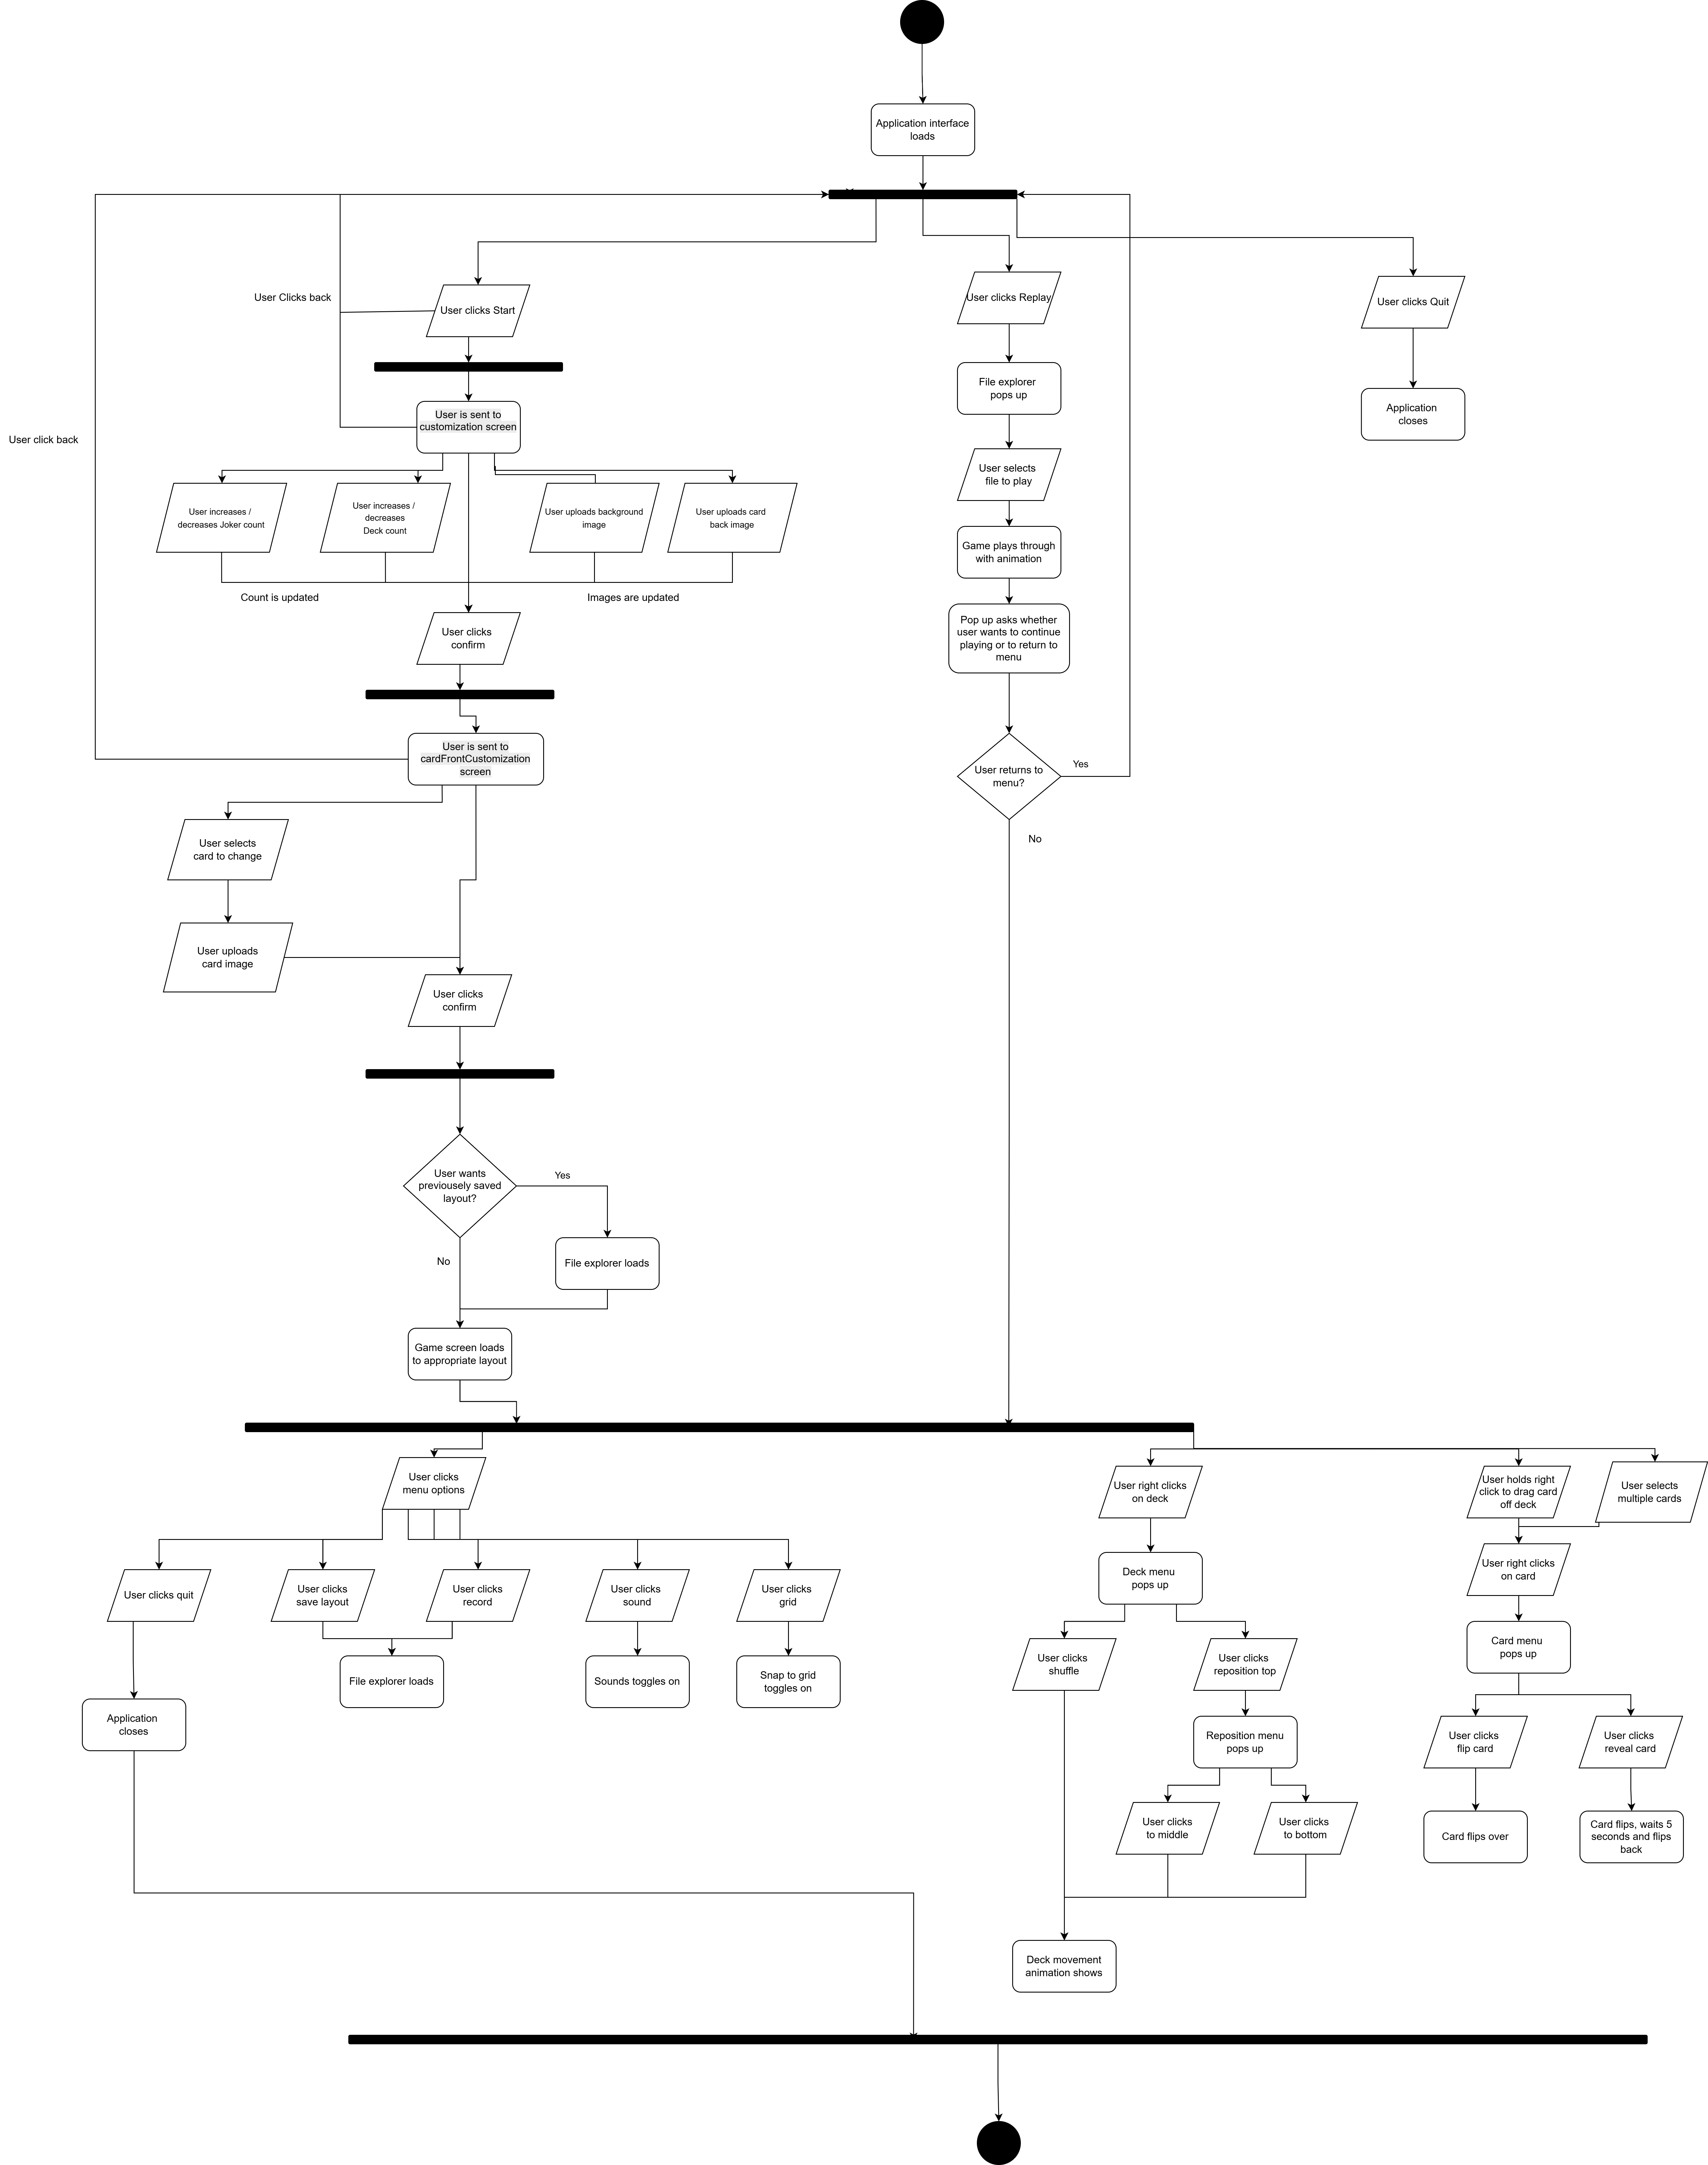
\includegraphics[width=1\linewidth]{assets/state-diagram.jpg}
				\caption{State Diagram}
				\label{fig:State Diagram}
			\end{figure}
			
			\clearpage
			
			This state diagram represents the user interaction flow within the card-based application interface. It outlines the application's behaviour from initial launch through various interactive states, including customization, gameplay, and termination. Upon entering the application, users are presented with a main interface that branches into several functional areas. These areas include customization options, file handling, and game playing. \\
			The customization process allows users to tailor the visual and structural elements of the gameplay environment, such as choosing their own images for cards and selecting number of jokers wanted. File handling provides a mechanism for loading custom images or previously saved content. When updating images, once file selection is complete, the user is shown the screen they were previously on again, but updated to display their image as required. The gameplay state supports a range of user interactions, including modifying card layouts, engaging with individual or multiple cards, and accessing game menu options. The game menu options include the ability to toggle sound, access replay, or exiting the application. Users may return to prior states, such as the customization screen, from various points within the workflow. \\
			Overall, the diagram captures the dynamic flow between user actions and application responses, highlighting the structure and interactive capabilities of the system without being bound to any single path or sequence. It provides a blueprint for understanding the user experience and the logical transitions that govern application behaviour.
			
			\clearpage
		
		\addcontentsline{toc}{section}{REFERENCES}
		
		\begin{thebibliography}{5}
			\bibitem{DS1} \emph{Software Engineering Group Projects}
			UI Prototype Design Specification.
			N Perry, F Sasso, N Spence, R Fraser, A Al-Samarrai, J Ball, W Shipp, P Sharma DS1 2.0 Release.
			\bibitem{SE.QA.05} \emph{Software Engineering Group Projects}
			Design Specification Standards (CS22120).
			C.W. Loftus SE.QA.05. 3.4 Release.
			\bibitem{Product Backlog} \emph{Software Engineering Group Projects}
			Product Backlog (CS22120).
			C.W. Loftus Product Backlog 1.4 Release.
		\end{thebibliography}
		
		\clearpage
		
		\addcontentsline{toc}{section}{DOCUMENT HISTORY}
	
	\section*{DOCUMENT HISTORY}
	
		\begin{center}
			\begin{tabular}{|l|l|l|l|l|}
				\hline
				Version               & Issue No. & Date                        & Changes made to Document                  & Changed by             \\ \hline
				\multirow{3}{*}{0.1}  & \#49      & \multirow{3}{*}{25/02/2025} & Added First draft Package diagram         & N.S.                   \\
				                      & \#50      &                             & Added system diagram                      & N.P.                   \\
				                      & \#52      &                             & Added mapping US to classes               & R.F., F.S.             \\ \hline
				0.2                   & N/A       & 26/02/2025                  & Created skeleton for document             & R.F.                   \\ \hline
				\multirow{2}{*}{0.3}  & \#86      & \multirow{2}{*}{11/03/2025} & Added introduction paragraph              & R.F.                   \\
				                      & \#127     &                             & Updated package diagram                   & N.S.                   \\ \hline
				0.4                   & \#35      & 12/03/2025                  & Reformatted \LaTeX\ version               & N.P.                   \\ \hline
				\multirow{9}{*}{0.5}  & \#177     & 18/03/2025                  & Added US1 design diagram and description  & R.F.                   \\
				                      & \#178     & 18/03/2025                  & Added US2 design diagram and description  & R.F.                   \\
				                      & \#179     & 18/03/2025                  & Added US3 design diagram and description  & R.F.                   \\
				                      & \#180     & 18/03/2025                  & Added US4 design diagram and description  & R.F.                   \\
				                      & \#181     & 18/03/2025                  & Added US5 design diagram and description  & F.S.                   \\
				                      & \#182     & 18/03/2025                  & Added US6 design diagram and description  & F.S.                   \\
				                      & \#184     & 18/03/2025                  & Added US8 design diagram and description  & N.S.                   \\
				                      & \#186     & 18/03/2025                  & Added US10 design diagram and description & A.A.                   \\
				                      & \#120     & 18/03/2025                  & Added US13 design diagram and description & R.F.                   \\ \hline
				\multirow{18}{*}{0.6} & \#54      & 19/03/2025                  & Added pseudocode for US1                  & R.F.                   \\
				                      & \#61      & 19/03/2025                  & Added pseudocode for US2                  & R.F.                   \\
				                      & \#62      & 19/03/2025                  & Added pseudocode for US3                  & N.P.                   \\
				                      & \#63      & 19/03/2025                  & Added pseudocode for US4                  & J.B.                   \\
				                      & \#64      & 19/03/2025                  & Added pseudocode for US5                  & R.F.                   \\
				                      & \#65      & 19/03/2025                  & Added pseudocode for US6                  & A.A.                   \\
				                      & \#66      & 19/03/2025                  & Added pseudocode for US7                  & F.S.                   \\
				                      & \#67      & 19/03/2025                  & Added pseudocode for US8                  & A.A.                   \\
				                      & \#68      & 19/03/2025                  & Added pseudocode for US9                  & F.S.                   \\
				                      & \#69      & 19/03/2025                  & Added pseudocode for US10                 & F.S.                   \\
				                      & \#70      & 19/03/2025                  & Added pseudocode for US11                 & F.S.                   \\
				                      & \#71      & 19/03/2025                  & Added pseudocode for US12                 & N.S.                   \\
				                      & \#72      & 19/03/2025                  & Added pseudocode for US13                 & P.S.                   \\
				                      & \#73      & 19/03/2025                  & Added pseudocode for US14                 & N.P.                   \\
				                      & \#74      & 19/03/2025                  & Added pseudocode for US15                 & N.S.                   \\
				                      & \#75      & 19/03/2025                  & Added pseudocode for US16                 & P.S.                   \\
				                      & \#76      & 19/03/2025                  & Added pseudocode for US17                 & W.S.                   \\
				                      & \#77      & 19/03/2025                  & Added pseudocode for US18                 & P.S.                   \\ \hline
				\multirow{3}{*}{0.7}  & \#183     & 25/03/2025                  & Added US7 design diagram and description  & N.P.                   \\
				                      & \#187     & 25/03/2025                  & Added US11 design diagram and description & N.S.                   \\
				                      & \#188     & 25/03/2025                  & Added US12 design diagram and description & N.S.                   \\ \hline
				0.8                   & N/A       & 25/03/2025                  & Added system diagram description          & W.S.                   \\ \hline
				\multirow{9}{*}{0.9}  & \#87      & 01/04/2025                  & Added system diagram captions             & W.S.                   \\
				                      & \#185     & 01/04/2025                  & Added US9 design diagram and description  & P.S.                   \\
				                      & \#189     & 29/05/2025                  & Added US14 design diagram and description & F.S.                   \\
				                      & \#160     & 01/04/2025                  & Added US15 design diagram and description & A.A.                   \\
				                      & \#190     & 01/04/2025                  & Added US16 design diagram and description & A.A.                   \\
				                      & \#162     & 01/04/2025                  & Added US17 design diagram and description & A.A.                   \\
				                      & \#56      & 01/04/2025                  & Added state diagram                       & R.F.                   \\
				                      & \#219     & 01/04/2025                  & Added state diagram description           & R.F.                   \\
				                      & \#186     & 01/04/2025                  & Added US11 design diagram and description & R.F.                   \\ \hline
				1.0                   & \#210     & 29/04/2025                  & Added US18 design diagram and description & F.S.                   \\ \hline
				\multirow{3}{*}{1.1}  & N/A       & 29/04/2025                  & Added system diagram description          & W.S.                   \\
				                      & \#88      & 30/04/2025                  & Updated package diagram                   & N.S.                   \\
				                      & \#51      & 06/05/2025                  & Class diagrams                            & F.S.                   \\ \hline
			\end{tabular} \par
		\end{center}
		
		\begin{center}
			\begin{tabular}{|l|l|l|l|l|}
				\hline
				Version              & Issue No. & Date       & Changes made to Document                   & Changed by             \\ \hline
				\multirow{3}{*}{1.2} & N/A       & 07/05/2025 & Update pseudocode and diagram descriptions & N.P.                   \\
				                     & \#223     & 07/05/2025 & Added class descriptions                   & N.S., A.A., W.S., P.S. \\
				                     & N/A       & 08/05/2025 & Final cleanup and proof reading            & N.S.                   \\ \hline
			\end{tabular} \par
		\end{center}
	
		\label{thelastpage}
	
\end{document}